%!TEX  root=./LIVRO.tex

\chapter{1. Fuga e transformação}\label{fuga-e-transformauxe7uxe3o}

\begin{figure}[H]
\centering
  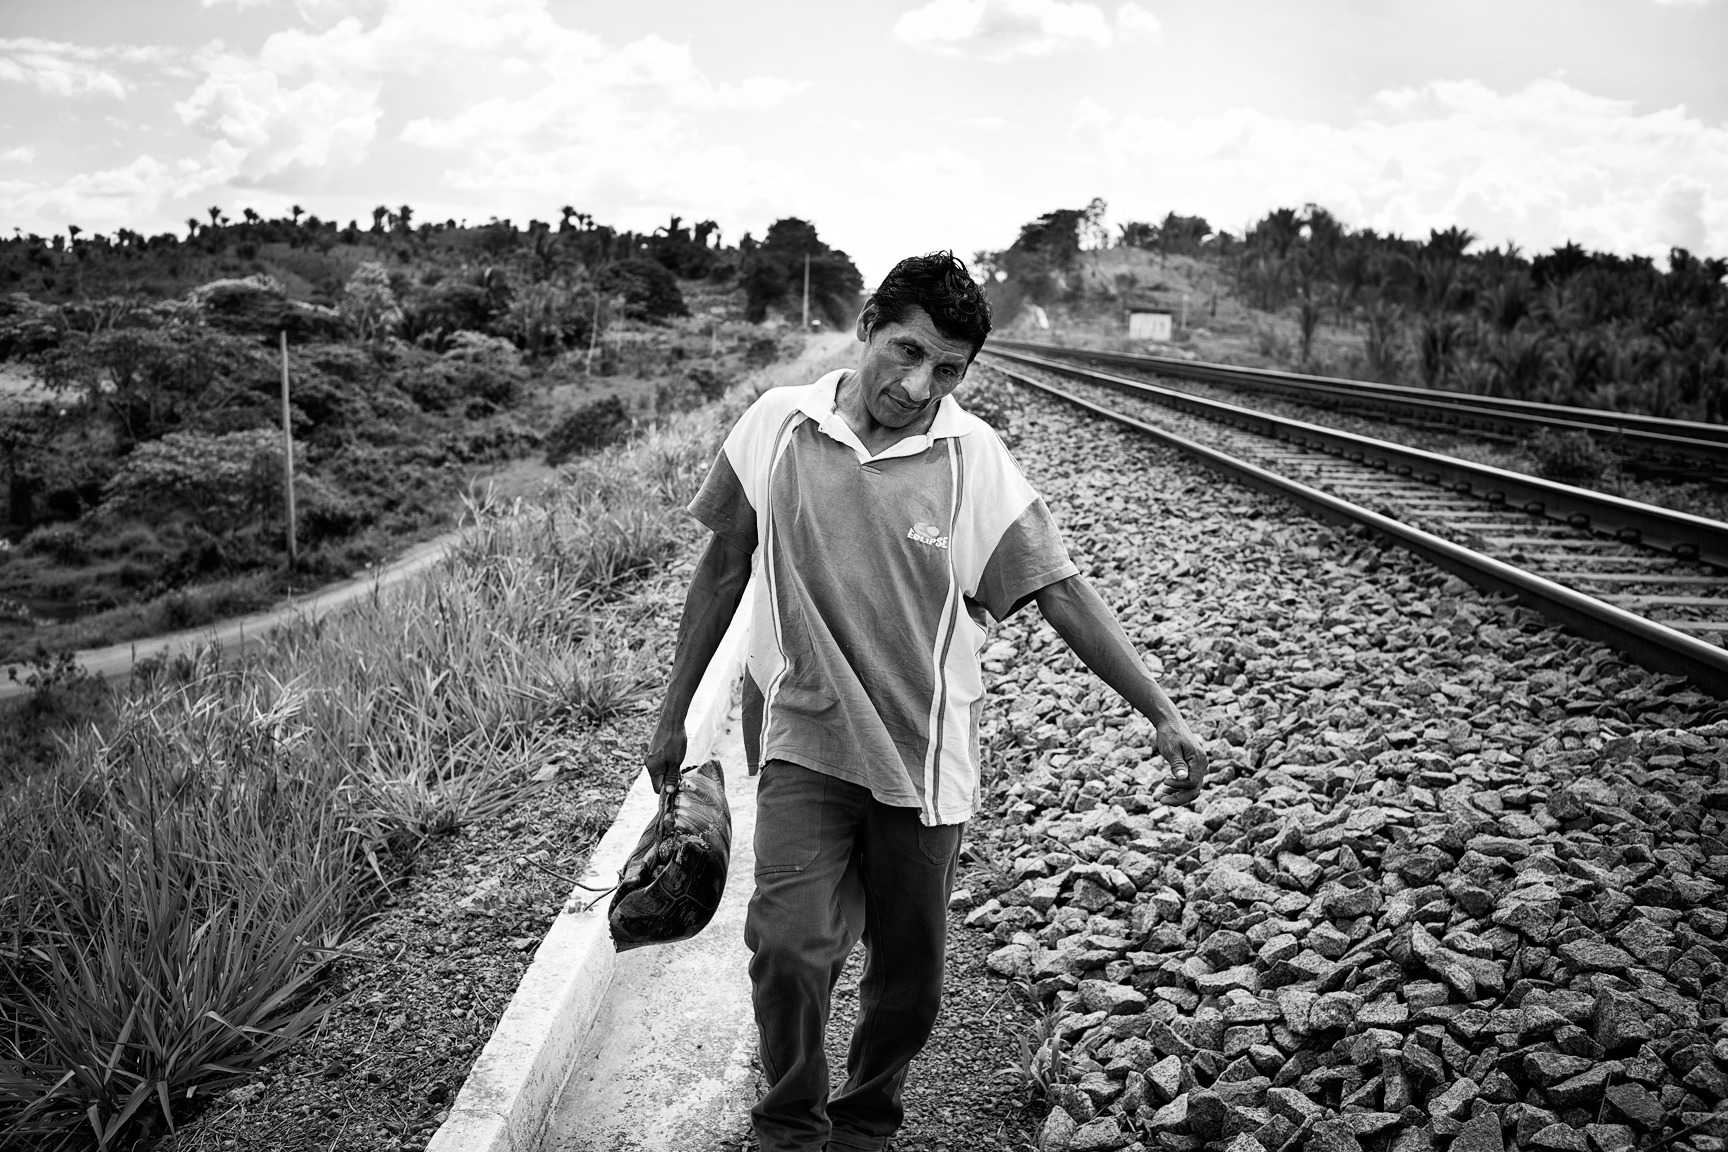
\includegraphics[width=\textwidth]{./imgs/Irakatakoa_426}
%\caption{}
\end{figure}

\noindent Os Guajá são um pequeno grupo de caçadores habilidosos, habitantes da
porção oriental da Amazônia, mais exatamente o noroeste do estado do
Maranhão. Andarilhos, desconheciam a navegação, ocupavam
predominantemente áreas isoladas próximas a babaçuais no interior da
floresta onde, de maneira dispersa, conseguiram se manter ``isolados''
até o fim da década de 1980, e existem pessoas em isolamento voluntário
até os dias atuais. Sempre ocuparam os topos e ramificações das serras
do Tiracambu e da Desordem, que formam parte da região oeste maranhense,
drenadas pelos rios Turiaçu (bacia do Turiaçu), Caru e Pindaré (bacia do
Mearim), e rios menores como o Turi, Turizinho, rio do Sangue, rio do
Peixe, além de inúmeros igarapés formadores e tributários, como Juriti,
Mão de Onça, Maronata, Presídio, Bandeira, Mutum, Aprígio, igarapé do
Furo, do Milho, Guariba, Aparitiua, dentre outros ainda menores. Por ali
os Guajá procuraram refúgio a fim de escapar da sede durante fugas,
quando resistiam ao contato (para detalhes sobre a hidrografia e
topografia, ver O'Dweyer, 2010, p.86).

Habitantes do que restou de floresta no estado do Maranhão, eles se
encontram na macrorregião da Amazônia Oriental e são falantes de uma
variante do Tupi"-Guarani em um subgrupo desta família linguística
composto por nove línguas: Emerillon, Wayãpi, Zo'é, Guajá, Anambé,
Ka'apor, Takunyapé, Turiwára e Amanayé (Rodrigues, 1984/85). Em sua
história, não tiveram aldeias permanentes e até o contato organizavam"-se
em pequenos coletivos, formados por uma ou duas famílias nucleares,
dispersos sobre um território também ocupado por outros povos indígenas
(Tenetehara e Ka'apor). Não dominavam cultivo agrícola algum, nem mesmo
milho ou mandioca, até o contato, e tal situação se modificou sobretudo
na última década passada, quando a população mais jovem era ``ensinada''
por funcionários da Funai a cultivar mandioca (basicamente para a
produção de farinha puba), além de milho, macaxeira, abóbora e arroz.
Portanto, as roças para os Guajá pertencem aos \emph{karai}, aos
não"-indígenas.

Antes de tudo, os Guajá são exímios caçadores. A caça é sua principal
atividade --- um tema que interessa a todos---, e é nessa atividade que as
pessoas depositam grande parte de seu tempo. Caçam diversas espécies de
aves e mamíferos; detêm uma técnica extremamente apurada para a caça de
mamíferos arborícolas, em especial cinco tipos de macacos (macaco"-prego,
cuxiú, capelão/guariba, cairara e mão"-de"-ouro/
macaco"-de"-cheiro). A caça em geral --- a de macacos, especificamente --- é
uma atividade que mobiliza toda uma aldeia: homens, mulheres e crianças.
Com tais características (caça e nomadismo), de tempos em tempos eles
aparecem nos meios de comunicação nacionais e internacionais como os
``últimos nômades caçadores"-coletores do Brasil'' e coisas do gênero.

O objetivo deste capítulo é apresentar essa história recente, baseada em
contatos e fugas, mortes na floresta e recomeços nas novas aldeias.
Histórias que os Guajá não nos deixam esquecer e são constantemente
rememoradas quando as pessoas falam de si, da família ou dos amigos.

Os Guajá provavelmente fazem parte de um histórico conjunto populacional
Tupi Oriental, assemelhando"-se em diversos aspectos não apenas a seus
vizinhos mais próximos (os Ka'apor e Tenetehara), mas a outras
sociedades do leste amazônico como os Asurini, Araweté, Parakanã e
Aikewara, por exemplo. ``Um complexo populacional que se estendia desde
as matas do médio Xingu até as bacias dos rios Capim, Acará, Gurupi e
Pindaré'' (Viveiros de Castro 1986, p. 137--139). São povos que
historicamente ocuparam a \emph{terra firme} e que, ao sofrerem pressões
de outros povos (das chamadas ``sociedades de \emph{várzea}'' cujo
domínio da cerâmica e técnicas de domesticação de planta era notório ---
ver Heckenberger et al. 1998; Neves 1999), foram forçados à dispersão.
Populações como os Wayãpi, Assurini, Parakanã, Tenetehara, Zo'e,
Ka'apor, Amanajós, Anambé, dentre outros, que fugiram ou desapareceram
(Viveiros de Castro 1986: 139; Gallois 2013; Forline, 1997, p. 29).

``Humanos'', como encontrado entre tantos povos ameríndios, é a tradução
para \emph{awa} e funciona como um marcador enunciativo de uma condição
de pessoa (Viveiros de Castro 2002: 371). Nos dias atuais, a depender da
aldeia, se autorreferem como ``Awá'', ``Guajá'' (nome que apareceu no
contato com o Estado Brasileiro) e ``Awá-Guajá'' (mais utilizado nos
últimos anos); é difícil precisar uma designação ``oficial''. O fato é que
no momento atual, em que ocorrem mutirões para tirar carteiras de
identidade, as pessoas escolheram o nome ``Awá"-Guajá'' para constar em
seus documentos. Em outras situações, no entanto --- como em reuniões com
não"-indígenas (\emph{karai}) ou com os Guajajara (\emph{kamara}) ---,
podem fazer uso de ``Guajá'' como nome do povo. Noto aqui que a
autodenominação ``\emph{awa}'' é também utilizada por outros povos de
variante Tupi"-Guarani, como os Ka'apor e Asurini. Embora Balée afirme
que sua autodenominação é \emph{Ka'apor}, o termo \emph{awa} também
funcionaria nesse contexto como sinônimo de pessoa, sobretudo com a
conotação ``alguém''. O termo \emph{awa}, lembra o autor, ``está
relacionado com os termos inflexivos referentes a ``pessoa'' e ``povo'' em
várias outras línguas Tupi"-Guarani'' (Balée, 1998). Os Asurini do Xingu
também se autodenominam \emph{awaete}, traduzido por ``gente de verdade''.
\emph{Awa}, nesse caso, teria o mesmo significado que entre os Guajá:
``humanos'', e o sufixo \emph{ete} seria um enfatizador traduzível, no
caso, Asurini e outros Tupi"-Guarani por ``verdadeiro'' ou ``muito'' (Müller,
1993). Na língua Guajá o sufixo enfatizador também seria \emph{-te}
(tal o \emph{ete} asurini), tributários do conhecido sufixo
intensificador/autentificador Tupi \emph{ete}. \emph{Awatea} refere"-se,
grosso modo, à humanidade próxima, ``gente de verdade'', em oposição,
por exemplo, a \emph{awa mihua} (``gente braba''), designativo atribuído
aos pequenos grupos que vivem em isolamento na mata, os chamados
``isolados''. Em linhas gerais, pessoas que partilham língua e hábitos
semelhantes, porém distantes no parentesco, no espaço e na história, não
são reconhecidas como \emph{awatea} (``gente de verdade''). Apesar de hoje
em dia serem utilizadas as formas ``Guajá'', ``Awá"-Guajá'' e ``Awá'' ---
uma vez que nas próprias aldeias, a depender da terra indígena e do
contexto enunciativo, os nomes variam ---, por uma economia textual opto
por utilizar a maior parte do tempo o termo \emph{Guajá}, acompanhando
outros autores (Balée 1994, 2013; Cormier 2003, Forline 1997).

\section{Caçadores}

\emph{Watama'a aria}, ``nós somos caçadores'', afirmações desse tipo são
comuns entre as pessoas de diferentes aldeias. Tal \emph{condição} é
expressa pelo vocábulo \emph{watama'a}\footnote{\emph{Aria} = nós que
  exclui o interlocutor (exclusivo), muito comum em diversas línguas
  indígenas.}, cuja tradução literal é ``aquele que caminha''. Como
veremos aqui, ``andar'' e ``caçar'' são formas que podem ser expressas pelo
mesmo verbo: \emph{wata}. Os Guajá caçam na mata, dormem na mata e
passam longas temporadas na floresta, mesmo na época das chuvas. As
aldeias, tal como experimentam hoje, são resultado de uma reengenharia
social empreendida pelo contato, cujo resultado foi a reunião de
diversos grupos locais anteriormente dispersos. Muitas das famílias que
hoje vivem juntas não se conheciam pessoalmente antes do contato
oficial. As cinco aldeias existentes foram criadas a partir desta
máquina estatal de contato que marcou a ocupação da Amazônia indígena
brasileira durante o período militar, sobretudo no seu fim no decorrer
da década de 1980, quando a maior parte dos Guajá foram contatados.

Trata"-se de um desses grupos Tupi"-Guarani do leste Amazônico,
caracterizados por uma baixa complexidade material e ritual em que
elementos como a fala e o canto, cosmologia e escatologia, dentre
outros, tomam o lugar de uma economia de símbolos e práticas rituais
(Viveiros de Castro, 1986, p. 23). Uma gente para a qual é mais fácil
produzir uma ``lista de ausências'' de elementos ``típicos'' (Viveiros
de Castro 1986, p. 47) dos povos indígenas ameríndios do que evocar uma
parafernália material que os distinga de outros povos. No que concerne à
cultura material, os Guajá não produzem cerâmica ou cestaria; seu
artesanato tradicional se resume a pequenos cocares e braceletes com
penas de tucano utilizados em um momento ritual específico; a redes e
tipoias de fibras de tucumã (ou tucum); suas casas, até o contato, eram
tapiris na floresta; não praticavam agricultura; arcos e flechas são os
únicos artefatos produzidos em profusão cotidianamente. Com exceção das
belas redes de tucum, que abrigavam por vezes uma família inteira em uma
única peça (o casal e seus filhos pequenos), e uma estrutura com moquém,
uma aldeia Guajá não possuía pátio central, espaços diferenciados de
acordo com sexo ou classe de idades, caminhos e saídas para as roças ou
jardins, e era constituída por pouquíssimas pessoas, às vezes reunidas
em uma única casa.

Quanto aos marcadores sociais, os Guajá não se diferenciam muito dos
outros Tupi"-Guarani orientais como, por exemplo, os Araweté. Elementos
como ``divisão do trabalho fluida'', ``simplicidade dos sistemas de
prestação e contraprestação cerimoniais ou profanos'', ``morfologia
espacial aparentemente caótica'', ``repertório mínimo de papéis
sociais'' e ``ausência de qualquer segmentação global'' (\emph{idem}) parecem
compor o quadro das relações cotidianas Guajá. A diferença destes para
outros Tupi do leste Amazônico está, sem dúvida, em uma secular ausência
de agricultura em sua história, além do papel preponderante das mulheres
nas atividades de caça, como veremos aqui.

Sabemos sobre outras populações da mesma região que, movidas por
diferentes fatores, abandonaram as aldeias e se estabeleceram na mata,
com a vida baseada em caça e coleta e um ou outro cultivo agrícola. Nos
trabalhos de Viveiros de Castro sobre os Araweté (1986) e de Fausto
sobre os Parakanã (2001), encontra"-se que nem o abandono da aldeia
permitiu que essas pessoas deixassem totalmente a agricultura (da mesma
forma os Huaorani do Equador --- ver Rival 2002). Os Araweté mantiveram o
milho, enquanto os Parakanã Ocidentais, mesmo em um \emph{trekking}
permanente, resistiram com o cultivo da mandioca em seu sistema de vida.
Os Guajá, diversamente, pelo menos durante todo o século \versal{XX}, não se
familiarizaram com nenhum item de roça, e não há menção de conhecimento
sobre agricultura em sua história; nem mesmo os velhos se lembram de um
dia seus ``avós'' terem plantado o que quer que fosse. Em contraponto a
este passado, as pessoas hoje em dia estão sendo instruídas pelos
funcionários dos antigos Postos Indígenas (doravante, \versal{PIN}) para plantar
principalmente roças de mandioca para produção de farinha, alimento pelo
qual têm grande apreço e não conheciam até o contato. Muitos contam que
os mais velhos, ao se aproximarem da \versal{FUNAI}, se recusavam a comer farinha
(\emph{taramỹ}), pois pensavam tratar"-se de terra (\emph{wy}). Apesar de
todas as aldeias praticarem agricultura hoje em dia (e sempre com a
ajuda de mão"-de"-obra contratada pela \versal{FUNAI}), a ``lógica'' de ação ainda é
baseada na caça, e pelo menos nas aldeias em que vivi as pessoas ainda
estão dispostas a trocar uma colheita coordenada pela \versal{FUNAI} pela mera
suspeita da existência de uma vara de porcos, ou um bando de capelães,
muitas vezes acarretando perdas significativas na produção agrícola. Por
essas características, dentre outras que ainda veremos no decorrer do
livro, os Guajá são considerados por correntes ecológicas na
antropologia parte de um grupo de pessoas (cada vez mais raro no mundo
contemporâneo) definidas --- um tanto genericamente --- como
``caçadores"-coletores'' (Lee and Daly, 1999).

Tais observações remetem a uma discussão clássica da etnologia
americanista referente à existência (e pertinência da ideia) de povos
caçadores"-coletores na América do Sul tropical. Na história da etnologia
sul"-americana, por exemplo, dentre tantos outros coletivos como os
Nambikwara e os povos de língua Maku, duas sociedades, ambas
Tupi"-Guarani, foram constantemente citadas como paradigmáticas quando o
tema era caça e coleta: Aché e Sirionó. Por terem sido algo como um
``modelo'' nessa discussão, os Aché despertaram o interesse de
sociobiologistas pela busca de revelar como o grupo conservara
``características do Paleolítico'' em pleno século \versal{XX} (Hill \& Hawkes
1983). Tais pesquisadores classificaram os Aché algo como sobreviventes
da pré"-história, a despeito da revolução neolítica e de a agricultura
ser amplamente praticada na Amazônia (Roosevelt 1992: 202). Em diversas
análises (cf. Lévi"-Strauss 1970: 121--139; Service 1971; Viveiros de
Castro 1986: 106; Balée 1999; Fausto 2001), os Sirionó (assim como os
Aché) estão presentes como fiéis representantes desses pequenos bandos
de caçadores nômades, dotados de uma estrutura social quase amorfa.
Sirionó, Aché e também Guajá desenvolveriam aquilo que Clastres
criticamente denominou ``economia da miséria'' (2004 {[}1976{]}: 178).

A Amazônia e outras terras baixas sul"-americanas eram vistas como
universos puramente ``naturais'', onde os povos mais aptos a ocupar esse
ecossistema seriam os chamados caçadores"-coletores (Balée 1992). De
alguma forma, uma vez que durante milhares de anos da história humana em
algum momento a humanidade viveu de caça e coleta, gradativamente
substituídas pela agricultura há cerca de 10.000 a 5.000 anos (Neves
1988 \emph{apud} Balée 1992), cientistas com diferentes orientações, como se
estivessem à procura de nossas origens, ``consideram que a pesquisa
sobre caçadores"-coletores modernos, tais como os da Amazônia, poderia
elucidar padrões de utilização de recursos por parte de nossos
antepassados pré-agrícolas'' (Balée 1992). Tal ideia é utilizada pela
ciência a fim de ilustrar quase que uma espécie de ``elo perdido'' e
sustenta que a humanidade, em algum período de sua história, foi por
completo formada por povos caçadores"-coletores (Ingold 2003: 123).

\section{Povo do cocal}

Os Guajá estão inseridos em uma área onde espécies botânicas utilizadas
como recursos primários só se tornaram dominantes e/ou frequentes em
regiões onde havia intervenção humana direta --- mais exatamente a
agricultura ---, e boa parte dos espaços supostamente ``naturais'' pode
ter tido um passado agrícola, conectando povos sem agricultura a uma
cultura de capoeira (Balée 1992). E, também, as matas amazônicas estão
longe de ser ``primordiais'', diferentemente das ``teorias
adaptacionistas em ecologia cultural, que assinalam que grupos indígenas
da Amazônia se adaptam às condições e respondem aos limites
meio"-ambientais'' --- a floresta e outros \emph{habitats} amazônicos não
são somente de origem ``natural''. Em suas estimativas, o autor
considerava que ``pelo menos 11,8\% da mata de terra firme na Amazônia
brasileira é antropogênica'' (Balée 1987). Como um exemplo, Balée
seleciona justamente o caso Guajá:

\begin{quote}
\emph{Os Guajá são um dos últimos grupos forrageiros da América do Sul.
(\ldots{}) Tradicionalmente, procuravam comida em grupos de 5 a 10
pessoas em uma mata dominada, na sua maior parte, por árvores das
famílias da Castanheira"-do"-Pará, beru, faveira e abiu. Nunca derrubaram
ou queimaram a mata, fazendo seus acampamentos temporários
exclusivamente em cocais. (\ldots{}) Os cocais onde os Guajá acampam e
percorrem contêm, praticamente sempre, vestígios de aldeias e roças
antigas de outros grupos indígenas da região, como os Urubu"-Kaapor, que
habitam na fronteira leste de suas terras (\textbf{Balée 1987 citar a
página}).}
\end{quote}

Por terem sofrido um processo de ``perda'' do domínio agrícola devido a
efeitos de guerras, epidemias e colonização, adotaram um estilo de vida
baseado na caça e coleta (Balée 1994; 1999). O termo ``Regressão
Agrícola'', trabalhado por Balée, é utilizado a fim de ilustrar a
transição de uma organização econômica ligada à horticultura para a caça
e coleta, dois ``modos de produção'' complementares e compreendidos na
história como dois momentos diversos --- um deles, marcado por menos
pressões externas, o que favoreceria a sedentarização; e outro, em razão
das tais pressões, marcado pela mobilidade territorial, trazendo
mudanças à antiga vida sedentária que, deixada para trás, poderia ser
retomada de acordo com acontecimentos futuros. Embora alguns desses
caçadores"-coletores na América do Sul permaneçam com um conjunto de
plantas semidomesticadas , há a hipótese de que os vegetais cultivados
nessa transição ``desaparecem'' gradualmente; somente alguns gêneros são
mantidos, embora seu cultivo caia consideravelmente --- como é o caso do
milho entre os Sirionó (Balée 1994: 210).

É inescapável em análises como esta a atmosfera de arcaísmo, sugerida de
maneira indireta pela ideia de regressão. Rival, por exemplo, a critica,
ao afirmar que a tal ``passagem'' de um estado a outro é algo como uma
\emph{estratégia}, porém muito mais ampla e dinâmica do que uma resposta
à Conquista portuguesa ou espanhola na América do Sul (Rival 2002: 13).
Embora noções como ``forrageio ótimo'' (ver a crítica de Ingold 2002
pp.27--39) não terem sido operativas para esse autor como foi para outros
(Hawkes, Hill \& O'Conell 1982), a ideia de ``regressão agrícola''
supervalorizaria o ``sedentarismo'' em detrimento do tipo de vida que
povos como os Guajá levavam, baseadas em muitos deslocamentos pelo
território. É como se, uma vez que as pessoas pudessem ``optar'',
decidiriam não mais andar, numa correlação direta entre ausência total
de agricultura e mobilidade territorial. De acordo com a crítica de
Rival:

\begin{quote}
\emph{Balée, portanto, correlaciona a ausência de agricultura com a
mobilidade (territorial). Povos que cultivam intensivamente não possuem
grande mobilidade territorial; de modo inverso, povos que caçam e
coletam são altamente móveis. Embora eu concorde com sua insistência da
mobilidade ser considerada uma estratégia adaptativa histórica, ao invés
de somente uma imposição ambiental, lamento que o autor negligencie
dinâmicas históricas pré"-conquista desencadeadas por conflitos entre
populações nativas altamente móveis e outras menos móveis (Rival 2002:
13, livre tradução).}
\end{quote}

As plantas selvagens das quais dependem os Guajá são, por assim dizer,
semidomesticadas, uma vez que estão em áreas de capoeira, ou capoeiras
velhas, áreas antropizadas. Balée procura paralelos entre o conjunto
Tupi"-Guarani contemporâneo e sustenta três pontos: (1) os grupos \versal{TG}
forrageiros contemporâneos passaram por um processo de regressão
agrícola perdendo o domínio de todas as plantas domesticáveis, inclusive
do milho; (2) entre as plantas utilizadas, as diversas espécies de palma
ocupam papel central, tanto na alimentação quanto como matéria"-prima, e
(3) algumas dessas palmas --- como Jerivá e Mucajá (no Paraguai) na região
sudoeste do Brasil (Paraná) onde habitavam os Hetá, assim como Babaçu,
Inajá e Tucumã, todas presentes no território Guajá, são, devido a
predominância e frequência, indícios de presença pretérita de
horticultura (Balée, 1994, p.218). De acordo com esse autor, grupos
amazônicos que baseiam suas atividades no forrageio são capazes de viver
na floresta tropical sem o cultivo de roças graças a alguns recursos
essenciais (palmas e frutos, principalmente), que são subprodutos de
ocupação humana remota, e um padrão baseado na caça e coleta está
diretamente ligado à distribuição desses recursos no ambiente. A crítica
que fazemos é a mesma de Rival, pois nessas florestas bioculturais a
intencionalidade desses atos é sempre atribuída a uma ``inteligência''
passada, resultado de um conjunto de manejos anteriores (Rival 2002, p.
13).

Não cabe a este livro advogar contra modelos da ecologia política e da
ecologia histórica, e, independentemente das teses
regressivas/involutivas ou da pertinência em pensar uma mudança do
\emph{modo de produção} ``forrageiro'' para a agricultura, o objetivo
aqui é apresentar etnograficamente os processos de transformação pelo
qual vêm passando os Guajá. Esta suposta passagem entre modos de
produção tem sido experimentada pelas aldeias de uma maneira bastante
particular, como veremos mais abaixo; e, mais do que pensar uma mudança
no modo de produção (como sugerem certos autores), o que aparece aqui
são formas de se alimentar e agir como um novo tipo de gente. Uma gente
que sabe falar a língua dos \emph{karai} (os não"-indígenas) bastante
interessada em uma nova humanidade encontrada a partir do contato e que
faz uma leitura criativa do que seja o, assim chamado, ``trabalho'' na
roça.

Desde o contato, a \versal{FUNAI} operou uma transformação radical na vida das
pessoas. Além de uma sedentarização dos pequenos coletivos, podemos
falar em uma espécie de ``kit pacificação'', a partir do qual a farinha
de mandioca, as espingardas e os cachorros foram, muito rapidamente,
incorporados à vida nas aldeias e de muitas maneiras, como veremos nesse
livro, ganharam um papel de destaque\footnote{As armas de fogo, por
  exemplo, que foram introduzidas nas comunidades entre os anos de
  1970--1980 por funcionários da \versal{FUNAI} e toda sorte de agentes que
  participaram dos primeiros contatos, tornam"-se hoje uma ferramenta
  fundamental na caça, ao passo que, devido à lei federal do Estatuto do
  Desarmamento (Lei 10826 de 22 de dezembro de 2003), a mesma \versal{FUNAI} que
  introduziu armas e munições nas aldeias é impedida de fornecer tais
  itens às comunidades, não importando quão isoladas elas sejam.}. Junto
a esse processo de mudança, a ideia de que podem plantar sua própria
comida, frente a um passado de caça e coleta, aparece como um elemento
central e controverso, como veremos mais abaixo.

\section{Ecologia e Ferrovia }

A população Guajá é estimada em 420 pessoas (segundo o último censo que
realizei em 2013) que vivem em cinco aldeias (Juriti, Tiracambu,
\emph{Awá}, Aldeia Nova e Cocal/Guajá) distribuídas por três áreas
indígenas. Algumas aldeias adotam nomes análogos aos postos da \versal{FUNAI},
por isso não seriam nomes elaborados pelas comunidades, mas adequados
pelos postos. Apesar de ter conhecido todas elas, meu trabalho de campo
foi realizado nas aldeias Tiracambu, \emph{Awá} e Juriti, e durante os
anos de doutorado passei a maior parte do tempo de pesquisa na aldeia
Juriti.

%\textbf{Mapas}
\begin{figure}[H]
\centering
  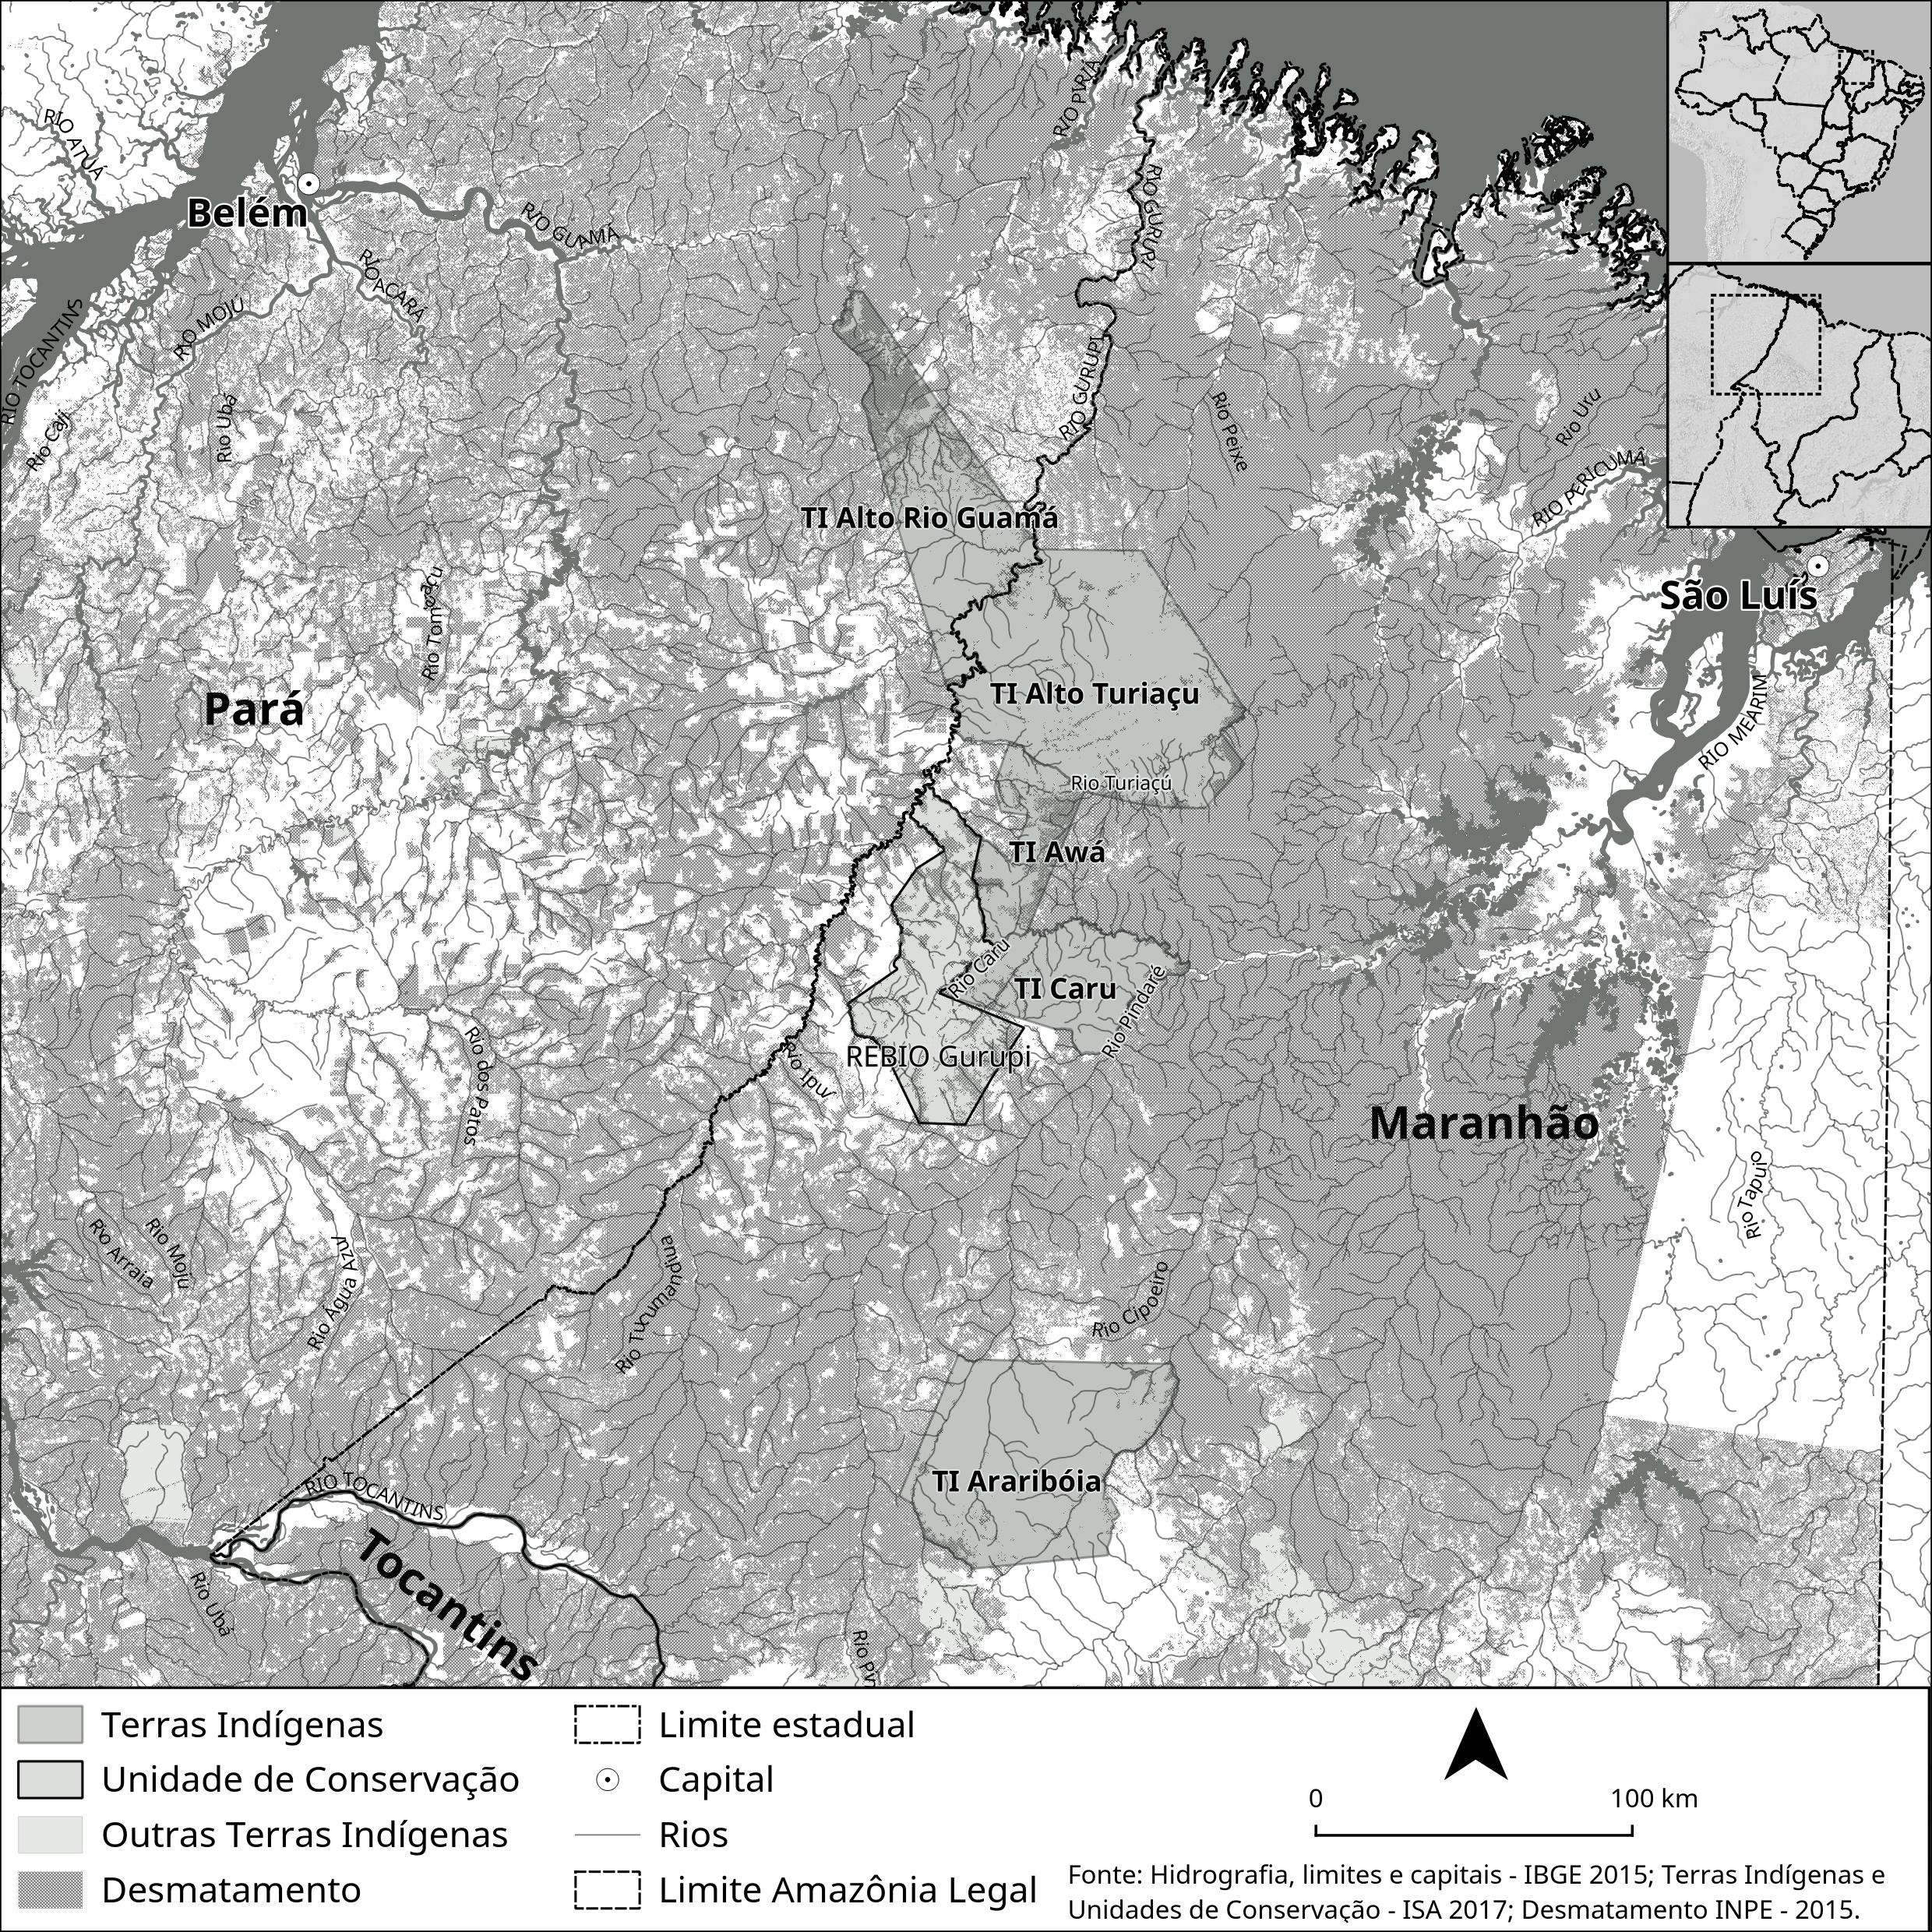
\includegraphics[width=\textwidth]{./imgs/mapa_livro_uira}
\caption{Mapa}
\end{figure}

À exceção da área indígena Awá (\versal{TI} Awá), onde se situa a aldeia Juriti,
os Guajá dividem suas \versal{TI}s com outros quatro grupos indígenas: Tenetehara
(Guajajara e Tembé), Ka'apor e alguns Timbira. No caso da área Carú, os
Guajajara estão em maioria, e possuem cinco aldeias, enquanto os Guajá,
na mesma área, formam três aldeias: \emph{Awá}, Tiracambú e Aldeia Nova.
Caso semelhante ocorre na aldeia Guajá, na terra indígena Alto Turiaçú,
área em que os Ka'apor estão em maioria. Nesta \versal{TI}, além dos Guajá e
Ka'apor, os Tembé (Tenetehara) também se fazem presentes, havendo ainda
um pequeno grupo Timbira. Nos último anos ocorreram casamentos de alguns
Guajá com Ka'apor ou Guajajara.

A área indígena Awá, onde se situa a aldeia Juriti, representa a única
área demarcada exclusivamente para os Guajá; a \versal{TI} Alto Turiaçú foi
pensada inicialmente com uma área Ka'ápor, e a área Carú, para usufruto
dos Guajajara. Atualmente, pela necessidade de estabelecer uma
convivência menos belicosa --- uma vez que parte dos dois povos divide o
mesmo território há décadas ---, os Guajá e Guajajara da \versal{TI} Carú procuram
estabelecer alianças políticas, principalmente frente às reivindicações
dirigidas à \versal{FUNAI}/Funasa. No entanto, ao mesmo tempo algumas pessoas das
aldeias Guajá observam que tais alianças caracterizam uma tentativa de
controle dos Guajajara sobre as decisões dos Guajá, inclusive com
propostas de alguns Guajajara chefiarem postos indígenas de aldeias
Guajá.

Desde os últimos 150 anos estima"-se que estejam nos arredores dos rios
Pindaré, Turiaçu e Gurupi, tendo este último rio sua área de
predominância na porção oeste do Maranhão. Essa região em que vivem tem
como limite o Rio Gurupi à oeste, o Oceano Atlântico ao norte, o alto
curso dos rios Pindaré, Grajaú e Gurupi ao Sul e, à leste, a margem
esquerda do Rio Mearim; nenhum desses rios é tributário do Amazonas.
Além dos Guajá, vivem na região os Ka'apor (Urubu), Tembé e Guajajara
(Balée, 1994, p. 10), dividindo"-se em três áreas contíguas: ao sul, a
Terra Indígena (\versal{TI}) Carú, com 172.600 ha ocupados conjuntamente com os
Guajajara; ao norte, a \versal{TI} Alto Turiaçu, com 530.500 ha, em companhia dos
Ka'apor e alguns Tembé; e, entre as duas, a \versal{TI} Awá, com 118.000 ha
(Cormier, 2000, p. 11). Além dessas três, alguns indivíduos habitam a
Terra Indígena Arariboia (Guajajara) e a \versal{TI} Alto Rio Guamá (dos Tembé),
contígua à \versal{TI} Alto Turiaçu (Cormier, 2000, p. 11).

A porção de floresta amazônica no \versal{MA} é um cenário com alto grau de
pressão antrópica, e a vida desses coletivos se desenrola na única
região de floresta tropical que ainda resta no estado, formando um
conjunto de terras indígenas e uma Unidade de Conservação que estão na
lista das mais desmatadas da Amazônia Continental. De acordo com estudos
recentes (Martins \& Oliveira 2011), as áreas indígenas são as únicas
áreas de floresta que restaram a ser preservadas (ao lado da Reserva
Biológica do Gurupi) no estado do Maranhão. Trata"-se, na Amazônia, de
uma região com uma das porções mais expressivas em termos de riqueza de
espécies e endemismos, onde se localiza mais da metade do Centro de
Endemismo Belém (Martins \& Oliveira 2011, p.20) e se abrigam animais
ameaçados de extinção, como a ararajuba (\emph{Guarouba guarouba}), o
gavião real (\emph{Harpia harpyja}), araçari (\emph{Pteroglossus
bitorquatus bitorquatus}) e a jacupiranga (\emph{Penelope pileata}),
além de duas espécies de primatas da Amazônia oriental, o ``Cairara
Ka'apor'' (\emph{Cebus kaapori}) e o ``Cuxiú-preto'' (\emph{Chiropotes
satanás}), todos ameaçados de extinção. De acordo com o \versal{ICMB}io, das 46
espécies listadas por pesquisadores como ameaçadas de extinção na
Amazônia, mais de 50\% estão presentes no Centro de Endemismo Belém.

Além dos Guajá, Tenetehara e Ka'apor (povos de língua Tupi), no oeste do
Maranhão, mais ao sul, há ainda os Ramkokamekra"-Canela e
Apaniekra"-Canela, os Krikatí e Pukobyê, falantes de línguas do tronco
Macro"-Jê; de modo geral, em toda a região oeste do estado do Maranhão há
porções ocupadas por povos indígenas. Tal região é composta por cidades
antigas como Pindaré"-Mirim, pelo surgimento de novas aglomerações ao
longo das Rodovias \versal{BR}"-316 (Belém"-Teresina) e \versal{BR}"-010 (Belém"-Brasília) e
pelo rápido crescimento de outras, como é o caso de Santa Inês. Trata"-se
de uma região onde migrantes do nordeste do País e do próprio Maranhão
promoveram uma ocupação à base de unidade de produção familiar,
sobretudo a partir da agricultura de corte e queima, que até hoje é
praticada com intensidade. Trata"-se de uma grande área (compreendida
pelas microrregiões do Gurupi, Pindaré, Imperatriz, Alto Mearim e
Grajaú) marcada por um rápido crescimento populacional e uma
avassaladora ocupação territorial (Diniz 2005).

Todo o território Guajá incide na macrorregião onde foi implantado o
Projeto Carajás (\versal{PGC})\footnote{O Projeto Carajás, oficialmente conhecido
  como Programa Grande Carajás (\versal{PGC}),1 é um projeto de exploração mineral
  iniciado em 1980 na mais rica área mineral do planeta, pela Vale
  (antiga \versal{CVRD}). Estende"-se por 900 mil km², uma área que corresponde a
  um décimo do território brasileiro, é cortada pelos rios Xingu,
  Tocantins e Araguaia e engloba terras do sudeste do Pará, norte de
  Tocantins e sudoeste do Maranhão. Foi criado pela empresa estatal
  brasileira Companhia Vale do Rio Doce --- durante o governo Figueiredo ---
  quando Eliezer Batista era seu presidente (fonte:
  http://pt.wikipedia.org/wiki/Projeto\_Grande\_Carajás).}, cuja
ferrovia para transportar sobretudo minério de ferro foi inaugurada em
1985, fazendo com que o contato com grupos que viviam isolados (ou
\emph{arredios}, segundo a terminologia da época) fosse acelerado. Na
ocasião, os contatos com os grupos Guajá ainda estavam sendo iniciados,
e centenas de indivíduos sem contato morreram vitimados por doenças e
assassinatos provenientes do \emph{boom} populacional que houve na
região, propiciado pela construção da ferrovia. A Estrada de Ferro
Carajás (\versal{EFC}) cortou o território tradicional Guajá, provocando não
apenas a perda de suas terras, mas a dispersão e a morte dos animais de
caça e o fim de boa parte das florestas do oeste maranhense. Foi esse
mesmo fenômeno, aliado à concomitante ocupação da região, dado o
crescimento de vilas e povoados, que produziu a divisão de muitos grupos
locais, pelo que alguns remanescentes experimentam até os dias de hoje
uma vida sem contato com outros grupos.

O Projeto Carajás, que não afetou apenas os Guajá, mas cerca de 40
comunidades indígenas diferentes (Treece 1987), tem importância direta
na configuração socioespacial dos povos indígenas da região atualmente.
O impacto da estrada de ferro, inaugurada em 1985, é sentido pelos Guajá
não apenas pela presença física da ferrovia e o \emph{boom} populacional
decorrente (que continua se intensificando devido ao projeto atual de
duplicação da ferrovia), mas também pelos transtornos ecológicos que
modificaram as atividades de caça (Garcia 2014b). O impacto social (com
o adensamento populacional) forçou, por um lado, a fuga e dispersão às
cegas de muitos grupos locais que ali viviam, e por outro, nos últimos
20 anos, a concentração de pessoas (que até então viviam separadas) em
grandes aldeias com até 200 habitantes (como é o caso da aldeia
\emph{Awá}, na \versal{TI} Caru), algo que os Guajá não conheciam em sua história
até então. As poucas iniciativas de ajustes ao impacto do contato e ao
desastre ambiental, há tempos anunciado para a Amazônia Oriental, foram
mal administradas. Escândalos de desvios de verba do ``Programa Awá'',
projeto financiado pela mineradora (até então estatal) Companhia Vale do
Rio Doce (\versal{CVRD}), durante as décadas de 1980 e 1990, criado a fim de
mitigar os impactos de suas ações na região, deram a tônica da atuação
da \versal{FUNAI} até meados dos anos 2000.

Dado o impacto que a construção da estrada de ferro Carajás traria (e
trouxe) às comunidades indígenas em sua área de influência, foi
estipulado que parte dos recursos do projeto (\versal{US}\$ 300 milhões) seria
aplicada em programas de assistência para esses povos, em forma de um
convênio entre a \versal{FUNAI} e a antiga \versal{CVRD}. Uma das principais exigências
com relação à construção da ferrovia era a manutenção da integridade dos
territórios indígenas afetados e o desenvolvimento de iniciativas que
garantissem a qualidade de vida de seus habitantes. Além dos Guajá e
Guajajara, a ferrovia causou impacto em diversas outras comunidades,
como os Xikrin, Gavião, Ka'apor e Suruí, pelo que a \versal{CVRD} foi obrigada a
manter projetos de compensação.

No caso específico dos Guajá, esse convênio foi um fracasso, visto que
mais de 20 anos se passaram para que a \versal{TI} Awá (onde se encontra a aldeia
Juriti) fosse homologada, tempo suficiente para causar inúmeros
transtornos decorrentes das invasões e exploração ilegal desse
território. Enquanto isso, os programas de saúde que vieram com as
frentes de contato não se preocuparam com os riscos evidentes diante da
fragilidade das pessoas contatadas. A intenção parecia ser contatar a
qualquer custo, de qualquer maneira, no ritmo desejado pelas
empreiteiras. Os primeiros contatos, sem os cuidados necessários,
resultaram na morte de vários indivíduos, e entre 1976 e 1980 morreram
aproximadamente dois terços dos residentes do \versal{PIN} Guajá (o primeiro a
ser criado, ainda em 1976) por doenças introduzidas, principalmente
malária e a gripe. A contratação de terceiros também não foi realizada
sob critérios satisfatórios --- muitos funcionários novos e temporários da
\versal{FUNAI} não foram submetidos a exames médicos, situação que muitas vezes
trouxe enfermidades e óbitos. Fora isso, muitos observadores comentaram
que os recursos que outrora deveriam ser destinados aos objetivos
originais do convênio foram aplicados em infraestrutura para a própria
\versal{FUNAI}. Tempos depois foram criados outros convênios entre a \versal{FUNAI} e a
antiga \versal{CVRD}, desenvolvidos com interrupções e uma quantidade de recursos
menor do que o montante original. Passavam"-se períodos em que a \versal{CVRD}
apenas fazia pequenas caridades às comunidades Guajá. Um dos últimos
episódios, que veio à tona nos anos de 2001 e 2002, foi um grande desvio
de recursos da compensação por parte de um funcionário da antiga \versal{CVRD} e
o até então chefe do núcleo de apoio da Frente de Atração em Santa Inês.
Até ser descoberta a fraude a saúde Guajá ficou bastante comprometida, e
o dinheiro que deveria ser posto à disposição dos indígenas desapareceu.
Apesar de os fatos terem sido parcialmente apurados pela Justiça --- com a
demissão do funcionário da \versal{CVRD} envolvido no esquema e a condenação do
servidor da \versal{FUNAI} --- os Guajá nunca recuperaram o montante desviado. Até
os dias de hoje, todo os recursos que entram por meio da \versal{FUNAI} para as
aldeias Guajá são oriundos desse convênio.

Em decorrência desse megaempreendimento, a população regional cresceu
junto com o número de povoados ao longo da estrada de ferro. Tal pressão
demográfica aumentou o número de invasões nas áreas indígenas adjacentes
e intensificou o movimento dos trens da (agora) Vale, espantando a caça
e interferindo diretamente na vida de várias comunidades Awa"-Guajá e
Guajajara, já que a ferrovia margeia o perímetro sul da área indígena
Carú, junto ao rio Pindaré, como pôde ser observado no mapa acima.
Frente a tantos problemas, em várias ocasiões a estrada de ferro Carajás
foi fechada por um conjunto de povos insatisfeitos com o atendimento da
Sesai, \versal{FUNAI}, Vale ou demandas mais abrangentes ligadas aos indígenas.

O epílogo dessa história ainda não pode ser vislumbrado, mas os
desdobramentos não poderiam ser mais sinistros. Desde 2010 foi iniciada
a duplicação da \versal{EFC} --- levada a cabo por grandes empreiteiras, como a
Camargo Correa ---, empreendimento que passa beirando toda a extensão sul
da terra indígena Caru, e um novo convênio de compensação, além de um
gigantesco Plano Básico Ambiental (\versal{PBA}) está em curso incidindo nas
aldeias Guajá e Guajajara da \versal{TI} Caru, e na \versal{TI} Rio Pindaré (dos
Guajajara). Os recursos são volumosos, apesar de estarem aquém do real
impacto dessa obra na vida das pessoas. Além disso, como podemos ver no
mapa da região, a \versal{TI} Caru faz parte de um grupo maior de áreas que
deveriam ser protegidas, tal como vem sugerindo o grupo de trabalho
coordenado por Marlúcia Martins que congrega pesquisadores do Museu
Paraense Emílio Goeldi, e outras instituições governamentais e
não"-governamentais, através do que vem sendo chamado de ``Mosaico do
Gurupi'', uma área de gestão territorial. Diversas características
particulares de diversidade e endemismos, como já ressaltei,
justificaria pensar as \versal{TI}s e a Reserva Biológica (\versal{REBIO}) do Gurupi de
maneira conjunta. E mais, nesse mosaico, como se pode notar no mapa, a
\versal{TI} Awá é estratégica por ser o ``corredor'' que ligaria os dois blocos
de áreas protegidas, mais ao norte e mais ao sul. O \versal{PBA} da duplicação de
uma estrada de ferro voltado para uma única área indígena, quando a
estrada beira todo um Mosaico é --- além de incompleto e mesquinho ---
prejudicial ao funcionamento de todo um ecossistema que está entre os
mais ameaçados da zona tropical. Como investir em uma única área (Caru)
quando as outras quatro (Awá, Alto Turiaçú, Alto Rio Guamá e \versal{REBIO} do
Gurupi) estão desguarnecidas e completamente invadidas?

\section{Breve histórico }\label{breve-histuxf3rico}

Caçadores, habitantes das terras firmes do noroeste maranhense, os Guajá
se encontram nas franjas da floresta amazônica, em uma região de
ocupação Tupi"-Guarani que vai desde as matas do Xingu, sobe pelo
Tocantins, atravessa os rios Capim, Acará e Gurupi e chega até o
Pindaré. Gomes (1982), por exemplo, defende que uma das hipóteses mais
prováveis é a dos Guajá terem chegado na região na ``esteira'' dos
Ka'apor, grupo historicamente inimigo, que também migrava para a região
do rio Turiaçu. Até o século \versal{XIX} poderiam ser encontrados na porção
leste do estado do Pará e provavelmente atravessaram o Rio Gurupi
chegando ao atual Maranhão no final daquele século (ver Balée, 1994), e
lá encontraram os Tenetehara, possíveis descendentes dos Tupi da costa
maranhense. Sabe"-se também que estão desde o século \versal{XIX} pelas cabeceiras
dos rios Pindaré, Turiaçu e seus tributários (Gomes, 1982). Há outros
relatos que afirmam existirem grupos Guajá nas imediações do Pindaré e
Turiaçu há pelo menos 150 anos. Isso é discutido por Gomes (1985) e
retomado por Cormier (2003) ao defenderem que a menção mais antiga ao
nome deste povo data de 1853, notificado pelo presidente da província do
Maranhão, quando eles foram vistos às margens de afluentes do Caru e
Gurupi.

De acordo com o missionário José Noronha (1856), pelo menos 18 grupos
indígenas diferentes ocuparam as bacias Tocantins"-Araguaia na região de
encontro entre o baixo Tocantins e a ``boca'' do Araguaia (Balée, 1994,
p.25), na atual região em que hoje estão municípios como Imperatriz
(\versal{MA}), Marabá (\versal{PA}) e Paraupebas (\versal{PA}), desde
o ano de 1767. E na região da
margem esquerda do Tocantins, Noronha menciona um grupo, segundo ele
denominado \emph{Uayá}, que, de acordo com Balée (1994), podem ser os
antecedentes dos atuais Guajá (Balée, 1994, p.25). O problema do
argumento do autor reside tanto no fato de o termo ``Guajá'' não fazer
parte do léxico da língua nativa --- termo oriundo de fora --- como por
\emph{awa} (uma outra palavra da qual \emph{Uaya} pode ter surgido) ser
um vocábulo Tupi muito utilizado não só entre os Guajá, mas entre outros
povos de língua Tupi"-Guarani, como já mencionei.

Nimuendajú (1948) menciona alguns relatos, entre eles o de Francisco
Xavier Ribeiro Sampaio (1825), que em 1774 menciona entre os grupos
indígenas do baixo Tocantins os \emph{Uayá}. Outro autor apresentado por
Nimuendajú, Cezar Augusto Marques (1864), menciona os \emph{Ayaya}, um
povo ``selvagem'' que se encontrava nas imediações da estrada que ligava
Imperatriz a Belém. E, de acordo com Araujo Brusque (1862, p.12), os
\emph{Uaiara} (\emph{Guajará}, segundo Nimuendajú) podiam ser vistos no
alto curso do Rio Gurupi, mas não fixaram residência naquela região
(Nimuendajú, 1948). Anos depois, em 1873 foram noticiados novamente pelo
engenheiro Gustavo Luís Guilherme Dodt, que viajou pela região do Gurupi
na segunda metade do século \versal{XIX} e em 1873 publicou seu relato, reeditado
em Dodt (1939).

Sabemos que a vasta região entre os rios Xingu e Tocantins, ``na altura
do médio"-baixo curso de ambos, era ocupada por diversos grupos
Tupi"-Guarani'' desde o século \versal{XVII} (Nimuendajú, 1948, \emph{apud} Viveiros de
Castro, 1986), enquanto na margem direita do Tocantins estavam povos
não"-Tupi, como os Apinajé, Timbira e uns tais Acarajá"-pitanga. Os grupos
Tupi se encontravam na margem esquerda do Tocantins (Balée, 1994;
Noronha, 1856), e presume"-se que os Guajá sejam provenientes do que é
hoje o sudeste do estado do Pará, entre os rios Araguaia e o baixo curso
do Tocantins. Tal como outros povos Tupi"-Guarani, os Guajá também
parecem ser provenientes do interflúvio Tocantins"-Xingu, cujos alguns
povos migraram pelo leste amazônico (ex: Araweté, Parakanã e Asurini),
outros se deslocaram para o extremo leste (Ka'apor e Guajá) ou ainda se
encaminharam para o norte (Waiãpi) e meio"-norte (Zo'e) amazônico, tudo
ao longo dos últimos três séculos (Viveiros de Castro, 1986; Gallois,
1988; Balée, 1994). As causas para esta migração são desde guerras com
povos vizinhos até o encontro das populações nativas com a máquina
colonial que ocupou boa parte dos territórios indígenas. Balée cita,
para o caso Ka'apor, que uma epidemia de varíola e a guerra da
Cabanagem, ocorrida entre 1835 e 1836, acelerou a ida dos Ka'apor para a
bacia do Gurupi, no nordeste do Pará. Alguns povos provavelmente
originários deste conjunto Tupi"-Guarani podem ser hoje encontrados tanto
no Pará quanto no Maranhão, e a dispersão dos povos desta família
linguística, iniciada a partir do século \versal{XVII} como propõem alguns
autores (Viveiros de Castro, 1986; e Balée, 1994), tratou"-se talvez de
um dos últimos processos das sucessivas migrações que foram iniciadas na
pré"-histórica expansão Tupi (ver, por exemplo, Brochado 1984; Balée
1994; Noeli 1996; e Heckenberger \emph{et al}, 1998) e que configurou a
paisagem contemporânea não só dos grupos Tupi, mas de boa parte das
terras baixas sul"-americanas.

O registro da história Guajá é comumente baseado na de povos mais
conhecidos pela literatura etnológica --- como os Ka'ápor e Tenetehara ---
e feito por viajantes que circulavam na região. Foi assim, por exemplo,
que Curt Nimuendajú, \emph{in loco}, pôde esboçar as linhas do verbete
``Guajá'', publicado no \emph{Handbook of South American Indians}, Vol.3
(1948). Em 1919 ou 1911, os Tembé rastrearam e acossaram um pequeno
grupo Guajá desde a boca do rio Gurupí Mirim até suas cabeceiras que
acabou se rendendo aos atacadores. De acordo com Nimuendajú, segundo
relatos esses cativos logo morreram na aldeia Tembé de problemas
intestinais atribuídos à diferença da dieta deles e a dos Tembé. De
acordo com conversas que tive, na memória recente dos Guajá eles lembram
com temor o passado relacionado aos Tembé e afirmam que, nas histórias
dos mais antigos, os Tembé costumavam comer da carne dos antigos Guajá.
A histórica hostilidade entre os Guajá e os povos da região (Tenetehara
e sobretudo os Ka'apor) pode ser encontrada em relatos de autores como
Nimuendajú (1948, p.136) e Ribeiro (1996).

Diferente dos Ka'apor, que desde o século \versal{XIX} mantiveram contato com a
população não"-indígena, donde muitos se engajaram na extração da copaíba
(Balée 1994), o máximo de contato que os Guajá se permitiam além dos
conflitos armados era, segundo Balée, o assédio às roças dos Ka'apor. Em
1860, os Guajá estavam na bacia do Gurupi e, conforme alguns relatos,
assediavam as roças dos Ka'apor em busca de milho, batata doce, cará e
outros tubérculos, e não era incomum serem mortos pelos Ka'apor e Tembé
em situações como estas. Durante o século \versal{XX}, no entanto, algo
aconteceu. Mesmo sabendo da existência de roças e aldeias dos Ka'apor,
os Guajá perderam inclusive, como muitos de meus interlocutores me
lembraram, o interesse em consumir o milho. A mandioca, devido ao
dedicado processamento, já havia há muito sido abandonada, porém era
possível manter plantas de cultivo mais rápido e processamento mais
simples como o milho verde, como fizeram os Araweté em seus períodos de
\emph{trekking} (Viveiros de Castro, 1986, p. 49). É interessante notar
que, se os Guajá se interessavam pelo milho dos Ka'apor na segunda
metade do século \versal{XIX}, após algumas gerações o interesse foi se perdendo.
Piraima'ã, um homem velho da aldeia Juriti, contou"-me certa vez que em
sua juventude, bem antes do contato, encontrou uma roça de milho feita
pelos \emph{karai}. Sem saber como preparar aquele alimento, ele pegou
poucas espigas, mas imediatamente jogou fora pois não sabia como comer.

Em muitos relatos provenientes desde antigos presidentes das províncias
do Maranhão e do Pará, de acordo com autores como Gomes (1991) até
outros mais contemporâneos, como Nimuendajú e Beghin, os Guajá aparecem
como:

\begin{quote}
\emph{(\ldots) um povo nômade e arredio ao contato, com uma cultura material
muito simples em que se sobressaíam como traços marcantes os longos e
potentes arcos, o corte de cabelo em forma de cuia para ambos os sexos,
nenhum adornamento facial e o uso feminino de uma saia de fibra de
tucum, não muito diferente de uma tipóia de carregar bebê. No decorrer
dos anos foi"-se tomando conhecimento de outras características, a
inexistência da agricultura, a dependência alimentar da caça e da
coleta, a utilização integral do coco babaçu, a simplicidade de suas
aldeias/acampamentos, a presença de muitos xerimbabos, especialmente de
macacos capelães, e o tamanho pequeno dos grupos sociais (Gomes 1991:
355).}
\end{quote}

Com uma ressalva ao tamanho dos arcos, que nem sempre serão ``longos'' ---
embora também eu tenha encontrado na documentação registros de primeiros
contatos em que se mencionavam arcos de 1,80m ---, podemos concordar que
os Guajá se caracterizam historicamente por essa simplicidade material
apontada pelo autor. Além disso, nunca formaram algo como um coletivo
único. Não é de surpreender, portanto, que os ``Guajá'' como uma entidade
coletiva ainda seja um povo recém"-contatado, uma vez que o contato
dependerá de situações específicas que irão variar de grupo local para
grupo local, de família para família, ou mesmo de indivíduo para
indivíduo. Qualquer tentativa de remontar o passado, portanto, esbarrará
no fato de nunca terem se organizado em grandes aldeias. Os fragmentos
da história estão baseados em encontros fortuitos de um ou outro desses
pequenos coletivos não se abrangendo uma ``totalidade Guajá''.

\section{Contato e resistência}

\begin{quote}
\emph{Os karai (não"-indígenas) mataram minha esposa e meu filho. Eles
atiraram neles na mata. Atiraram com arma de fogo feita de ferro. Eu era
o pai. Quem morreu foi um antigo filho meu. Os karai o mataram com arma
de fogo. Nós corremos e eles foram atrás de nós e os mataram. Os karai
matam até crianças Awa! Mataram meu filho! Eu andei muito pela mata. Às
vezes era muito calor e sentia sede. De longe eu ficava observando os
karai. Via suas plantações de mandioca e milho. E pensava que um dia ia
matá-los. Andava muito pela floresta: a floresta é grande! Muitas vezes
eu estava tão perto dos karai que escutava o galo cantar. Por vezes eu
passava fome (Conversa com Karapiru, aldeia Tiracambu, 2013.
Tradução: Uirá Garcia e Marina Magalhães).}
\end{quote}

No terceiro dia do ano de 2015, foi noticiado por parte da imprensa
brasileira e internacional um contato realizado com um grupo Awá-Guajá,
composto por duas mulheres e um rapaz que fugiam pelas cabeceiras do
igarapé do Presídio, pequeno tributário do rio Pindaré, entre as Terras
Indígenas (\versal{TI}) Caru e Awá (no estado do Maranhão). O tal contato, melhor
definido como um encontro, uma vez que como é comum nesses casos as
pessoas em fuga aparecem como dispostas a se contatar, ocorreu nos
últimos dias de dezembro de 2014, e foi feito por um pequeno grupo
familiar que andava nas cabeceiras do referido igarapé, um local muito
utilizado para caçadas de todo tipo pela aldeia conhecida como Awá (\versal{TI}
Caru).

De acordo com a \versal{FUNAI}, tal como foi noticiado em portais de associações
como o Conselho Indigenista Missionário (\versal{CIMI} 2015) e outros sites de
notícias, as duas mulheres seriam Amakaria e Jakarewãyja, e o jovem
rapaz, filho de uma das mulheres, se chamaria Irahoa. Remanescentes de
um ``famoso'' grupo que resistiu ao contato na década de 1980, os três
chegaram ao fim da linha. Após décadas fugindo pelas matas e serras da
bacia do Pindaré, se viram encurralados sem perspectivas em um
território tido como dos mais ameaçados de toda a Amazônia Continental.
O contato foi feito por um grupo da aldeia Awá, e não por uma equipe da
Frente de Proteção Etnoambiental Awá-Guajá (\versal{FPEAG}), da mesma forma que
há quase uma década, em 2006, pessoas desta mesma aldeia localizaram e
contataram outra parte deste mesmo grupo --- Kara'ywãja e Wamaaxũa, mãe e
filho --- que vivia na mesma região.

Embora o contato oficial entre o Estado brasileiro e os Awá-Guajá tenha
se iniciado na década de 1970, já se tem notícias de contatos com grupos
desde 1943 quando um pequeno grupo apareceu às margens do rio Pindaré,
próximo a um posto que servia aos Guajajara, fugindo logo em seguida
(ver Gomes 1985). Em 1965, com a abertura da rodovia São Luís-Belém,
outro contato mal sucedido foi realizado com um grupo de 12 pessoas.
Trabalhadores da estrada avistaram esse grupo e acionaram a \versal{FUNAI}, que
levou cerca de 6,7 indígenas para o então \versal{PI} Gonçalves Dias (em parte
onde hoje é a \versal{TI} Rio Pindaré), e todas morreram em alguns meses (\emph{idem}).
Desde essa época até o final da década de 1980, as pessoas morreram de
tuberculose, sarampo, malária, disenteria e, sobretudo, gripe
(\emph{tata}, corruptela para ``catarro''). Todos os Guajá com mais de
25-30 anos guardam uma história sobre pessoas próximas vitimadas pela
gripe.

Os Awá vêm sendo contatados lentamente, e a assim chamada ``história do
contato'' pode ser definida como ``histórias dos contatos'', uma vez que
se encontra na documentação do \versal{SPI}/\versal{FUNAI} muitos relatos sobre pequenos
grupos de Awá-Guajá que fizeram contatos com agricultores e caçadores da
região desde a década de 1940. Muitas famílias apareciam ao contato
devido à invasão das áreas em que viviam e à falta de novos locais para
se deslocar. Em muitos desses encontros os Awá contraíam doenças como
sarampo e gripe, acarretando"-se óbitos muitas vezes de todo um grupo
local (Ver Gomes 1985 e Garcia 2010). Em relatos oficiais, desde 1966 há
presença dos Awá na região do Rio Pindaré, na altura do atual km 400 da
Ferrovia Carajás (Gomes 1984).

Oficialmente, o processo de contato com agências do Estado Brasileiro
teve início em 1973 pelas mãos dos sertanistas José Carlos Meirelles,
Florindo Diniz e Jairo Patusco, sendo que o primeiro contato só ocorreu
em 1976. O contato inaugural deu"-se com um grupo que se encontrava no
alto curso do Rio Turiaçú, grupo que originou o que hoje é a aldeia do
\versal{PIN} Guajá. Dos 56 indivíduos contados em 1976 só sobrariam 26 pessoas em
1980 muito doentes de malária e gripe. Vinte e seis anos se passaram, e
em 2002 esta população atingiu a marca de 67 pessoas (Gomes e Meirelles,
2002). A aldeia \emph{Guajá} talvez esteja dentre as que mais sofreram
as mazelas do difícil ciclo de contato, aldeamento e abandono que
ocorreram em boa parte das frentes de atração.

Semelhante a outros exemplos da política de contato e demarcação de
terras indígenas no Brasil, o caso Guajá foi outra tragédia. Ocorreram
diversas iniciativas de aproximação, sobretudo entre os anos 1970 e
1980. Além das frentes de atração, algumas famílias eram contatadas
``por acaso'' pois, por exemplo, estariam abatendo a flechadas os
cavalos de alguma fazenda com fins de subsistência. Esses indivíduos
contatados fora da visão das frentes de atração eram enviados para
aldeias já criadas pelo órgão indigenista e muitas vezes não mantinham a
menor relação com as pessoas da aldeia na qual viriam a ser alocados.
Sequer detinham o conhecimento necessário sobre a região para onde a
\versal{FUNAI} os levara. Outro fenômeno constante neste processo se refere a
muitas famílias Guajá que ``se contataram''.

Os Awá vivenciaram na década de 1970 um período crítico quando, como
ocorreu com outros povos indígenas, quase despareceram por completo. A
muitos deles só restava ou buscar o contato ou fugir ainda mais. O
contato dos Awá, portanto, como percebemos nos relatos da época, foi
realizado pelos próprios Awá-Guajá com os grupos locais, ao aparecerem
em vilarejos em busca de comida e socorro, tal como descreve José Carlos
Meirelles, que participou do primeiro contato:

\begin{quote}
\emph{A pressão feita pela sociedade envolvente nesta região com infiltrações
massivas de grileiros, caçadores e madeireiros profissionais faz com que
os índios Guajá procurem voluntariamente o contato nas mais diversas
áreas dos rios Carú, Turizinho, Alto Pindaré, Buriticupú, Gurupí e
afluente numa área de quase 2.000.000 hectares. Estes contatos
esporádicos com civilizados provocam contaminação, doença e morte, como
aconteceu na região entre o rio Carú e o rio Turiaçú (Meirelles, em
1973).}
\end{quote}

As pessoas se lembram de uma época em que viviam na floresta, mudavam"-se
constantemente de aldeias e passavam a maior parte do tempo caçando e
fugindo desse contato com os \emph{karai}. Não se lembram do passado com
nostalgia, mas com um misto de alegria, por terem vivido no mato, e
decepção, pela terrível experiência de fuga narrada nos anos que
antecederam os contatos. Eles defendem que os dias de hoje, com a
``farinha'' e a ``espingarda'', também são tempos interessantes. Porém
se queixam da proximidade compulsória que tiveram que estabelecer com os
\emph{karai} (os não"-indígenas), este grupo de pessoas que conheciam,
mas estrategicamente evitaram durante boa parte de sua história. Muitos
grupos que conviviam juntos no mato antes do contato acabaram se
separando, ao passo que outros que viviam sem contato passaram a ter uma
convivência próxima nas aldeias. Como exemplo, o grupo liderado por Amỹ
Paranawãja (hoje, com mais de 70 anos) e seu falecido marido Takwaxa'a,
contatado na década de 1980 e alocado na aldeia Tiracambu, circulou
tanto pelo distante Igarapé Água Preta quanto pela região do Igarapé do
Presídio e mantinha contato com outros grupos, como o de Ximira, que foi
contatado anos antes e alocado na aldeia \emph{Awá} (\versal{TI} Caru), e os de
Ajura e Juriximatỹa que vivem na aldeia Juriti (\versal{TI} Awá).

A estratégia de usar indivíduos contatados para os novos contatos, como
é comum em toda a Amazônia indígena, foi e ainda é utilizada aqui, à
diferença de que os últimos dois contatos (de 2006 e 2014) os Guajá
quiseram fazer sozinhos, sem ajuda estrangeira. Em um relato de Amỹ
Pirahỹ, mulher que mora na aldeia Juriti, percebemos o quanto grupos,
que até então estavam fugindo separados, se reuniam nessa fuga pela
sobrevivência, além de como Kamairu, um homem que já havia sido
contatado e morava nas proximidades do posto indígena \emph{Awá}, ajudou
no contato junto com a antiga Frente de Atração. A história se passa em
1989:

\begin{quote}
\emph{Eu não tinha medo dos karai (não"-indígenas) quando eu morava na
mata. Primeiro eu morava na mata, mas comia a macaxeira que era plantada
na roça dos karai. Os karai perceberam que tinha Awá pegando macaxeira e
resolveram ir nos pegar. Eles me procuraram. Eu fugia pela floresta,
pelo local onde vivíamos. Aí eu comia babaçu por lá. Era lá na mata,
perto do jurixi`ya (nome Guajá para o Igarapé Juriti). Estavam comigo
Takya, minha mãe (Amỹ Pirawãja), Muturuhũ, Pirama'ã, o Pira'ima'ã, que
ainda era bem jovem, e eu, que também era jovem. Antes de eu vir com a
Ajrua aqui no (posto indígena) Juriti, eu a vi, pela primeira vez, muito
longe daqui, na região do Igarapé Juriti. Meu pai estava caçando capelão
com Takya quando encontrou o grupo da Ajrua no mato e decidiram unir os
grupos. Alguns se afastaram e outros ficaram vivendo com eles, andando
juntos pela mata. Ficaram caçando juntos. Certa vez caçaram muitos
capelães. Pegaram um para ser seu animal de estimação. Coletaram mel
juntos: lascaram a árvore, derrubaram para pegar mel tiúba (jakajra),
que estava lá no alto. Derrubaram toda a árvore e ficaram tirando e
comendo mel juntos. Perguntaram uns para os outros onde ficavam suas
respectivas casas. --- Eu quero conhecer sua casa!, disseram uns aos
outros. E então Ajrua e Kamaraxa'a foram conhecer a nossa casa. E
ficamos todos juntos. Nós morávamos lá na mata e comíamos inajá. Nós
crescemos na mata. Ficamos muito tempo lá até que o Ruia (``Luis
Moreira'', funcionário da antiga Frente de Atração) nos pegou.} \emph{O
Kamairua veio do Awá e foi para onde estávamos com meu pai, o Muturuhũ.
Ele encontrou o Muturuhũ primeiro. E então o Muturuhũ disse que havia
mais gente. O Kamairua falou que queria encontrá-los. E nós estávamos na
mata, comíamos capelão assado e rasgávamos a carne dele no dente. Ele
chegou chamando: ---Uuuu, Uuuu! --- O que foi? --- Hã, aí vem um outro
Awá-Guajá, um homem! E o Muturuhũ nos explicou que estava trazendo um
outro Awá para nos encontrar e que este outro Awá já havia sido ``pego''
(contatado) pelos karaí (não"-indígenas). O Kamairua olhava para mim e
dizia: é mesmo, há outros Awá por aqui! --- O que vocês estão comendo?,
ele perguntou. Comíamos capelão e babaçu. Eu era acostumada a comer
babaçu. Mas não conhecia farinha. Eu ainda fiquei lá pelo mato e o
Kamairua foi embora com a esposa dele. Nós ficamos por lá e o Kamairua
vinha e voltava algumas vezes, com Muturuhũ. Um dia ele foi lá e levou
farinha, e comeu com babaçu. Eu não quis comer. Ele trouxe a farinha e
como eu não conhecia perguntei o que era. O Kamairua foi caçar macaco
com a gente. Matou macaco com a arma de fogo que ele tinha. Matou caça:
macaco"-da"-noite, mutum, inhambu. Ficamos lá e assamos no fogo. E
comemos. E ficamos muito tempo lá no mato. O Ruia foi atrás da gente e
falou para o Kamairua que queria nos levar para perto da casa dos karai
(posto indígena). Se não os levarmos, outros karai irão matá-los.}
\emph{Ah é!!! Então vamos sair daqui. E eles vieram nos buscar. E
ofereceram para nós banana e eu não queria comer porque não conhecia.
Ele disse que era muito gostoso. Eles comiam muita banana. Tinha muita
banana madura. Até que resolvemos experimentar e achamos gostoso. E
comemos de novo. Então Ruia falou que era bom comer com farinha, que era
muito gostoso. Aí eu comi. Todos nós comemos. Comemos tudo. Aí nós
construímos nossa casa lá. A casa era assim (aponta com a mão para um
tapiri). E o Kamairua veio nos dizer que era para ficarmos lá. Falou que
não era para irmos comer no mato e que iria matar capelão para nós. E
então ele matou capelão e trouxe, para que pelássemos. Nós fizemos o
fogo e o pelamos. E então abrimos a barriga do capelão, abanamos o fogo
e o colocamos para assar. E Kamairua ficou caçando para nós por um
tempo: matou capelão, cuxiu. Aí comíamos com farinha. Tinha muita
comida. Aí um dia de noite ele falou: fique por aqui. Eu respondi que
não iria fugir mais. Aí já havia outros Awá por aqui: o falecido Iharoa,
sua esposa Ajrua, e eu fiquei com eles. Ajrua vivia com seu primeiro
marido, Iharoa. Tinha a casa deles, onde moravam com sua filha
Panỹpinuhũ. (Conversa com Amỹ Pirahỹ, aldeia Juriti, 2013.
Tradução: Uirá Garcia e Marina Magalhães).}
\end{quote}

Durante esses anos, algumas famílias apareceram ao contato, muitas foram
assassinadas em emboscadas de fazendeiros e posseiros, outras morreram
de doenças, enquanto algumas, pelo que sabemos, ainda resistem em um
isolamento voluntário, recusando"-se a entrar neste jogo de contato com
os \emph{karai}.

A autonomia política representada pelos pequenos grupos familiares, sob
os quais se organizavam antes do contato (e de certa forma ainda
resistem nas pequenas subdivisões das aldeias atuais), fez com que o
processo de contato atravessasse a década de 1990 e se arrastasse até os
dias atuais com os grupos ainda sem contato nas \versal{TI}s Arariboia e Caru.
Desde o contato com os \emph{karai}, a vida se modificou bastante: nova
dinâmica espacial; nova alimentação; alianças compulsórias com grupos
locais até então rivais; nova língua, outras relações. Desde que foram
divididos nessas aldeias, há quase três décadas, essas pessoas não
souberam mais uma da outra, mesmo alguns deles sendo parentes
consanguíneos. Lembro também que a reunião desses diferentes coletivos
em aldeias transformou tais espaços em locais onde se falavam (ao menos
nos anos iniciais ao contato) diferentes variantes da mesma língua, como
atesta Magalhães (2013, p. 61), e conviviam ali diferentes dietas e
formas alimentares, alimentos que eram permitidos para alguns grupos
(como a carne de veado para mulheres) não eram permitidos a outros, e
com o decorrer dos anos essas trocas linguísticas e de hábitos foram se
uniformizando em cada uma das aldeias, havendo diferença, contudo, de
uma aldeia para outra. As considerações sobre o ``tempo do mato''
(\emph{ka'ape mỹna} ``antigamente na floresta''), acionadas a todo
momento pelas pessoas, são sempre lembradas a fim de mostrarem as
continuidades e as rupturas desde o contato com os agentes do Estado
Brasileiro, até os dias de hoje, quando as florestas estão sendo
invadidas por madeireiros e posseiros, e sua caça está cada vez menor. O
trauma experimentado nesse ``tempo do mato'' é atualizado hoje nas
memórias dessa época. Karapiru declarou"-me certa vez que, devido a seus
anos de fuga, ``morrera um pouco'' (\emph{manu} \emph{mixika'ĩ}) e por
isso não saberia mais cantar os cantos dos \emph{Karawara}.

Quanto aos Guajá ``isolados'' atuais (chamados \emph{mihua}), as
evidências apontam para quatro grupos ainda sem contato, vivendo pelas
matas das contínuas reservas Awá e Caru (municípios de Alto Alegre do
Pindaré e Bom Jardim) e Arariboia (municípios de Arame e Grajaú). Destas
quatro referências tem"-se a certeza de dois grupos confirmados e,
talvez, um terceiro (Vaz 2011). O grupo da \versal{TI} Arariboia é estimado em
até 60 pessoas (ver \versal{FUNAI} 2009), enquanto os outros são formados por
pouquíssimos indivíduos (algo como 3) e estariam um a oeste da área Caru
e outro na região do Igarapé Juriti, na \versal{TI} Awá.

\section{\emph{Wytyra}, as terras altas}

\begin{figure}[H]
\centering
  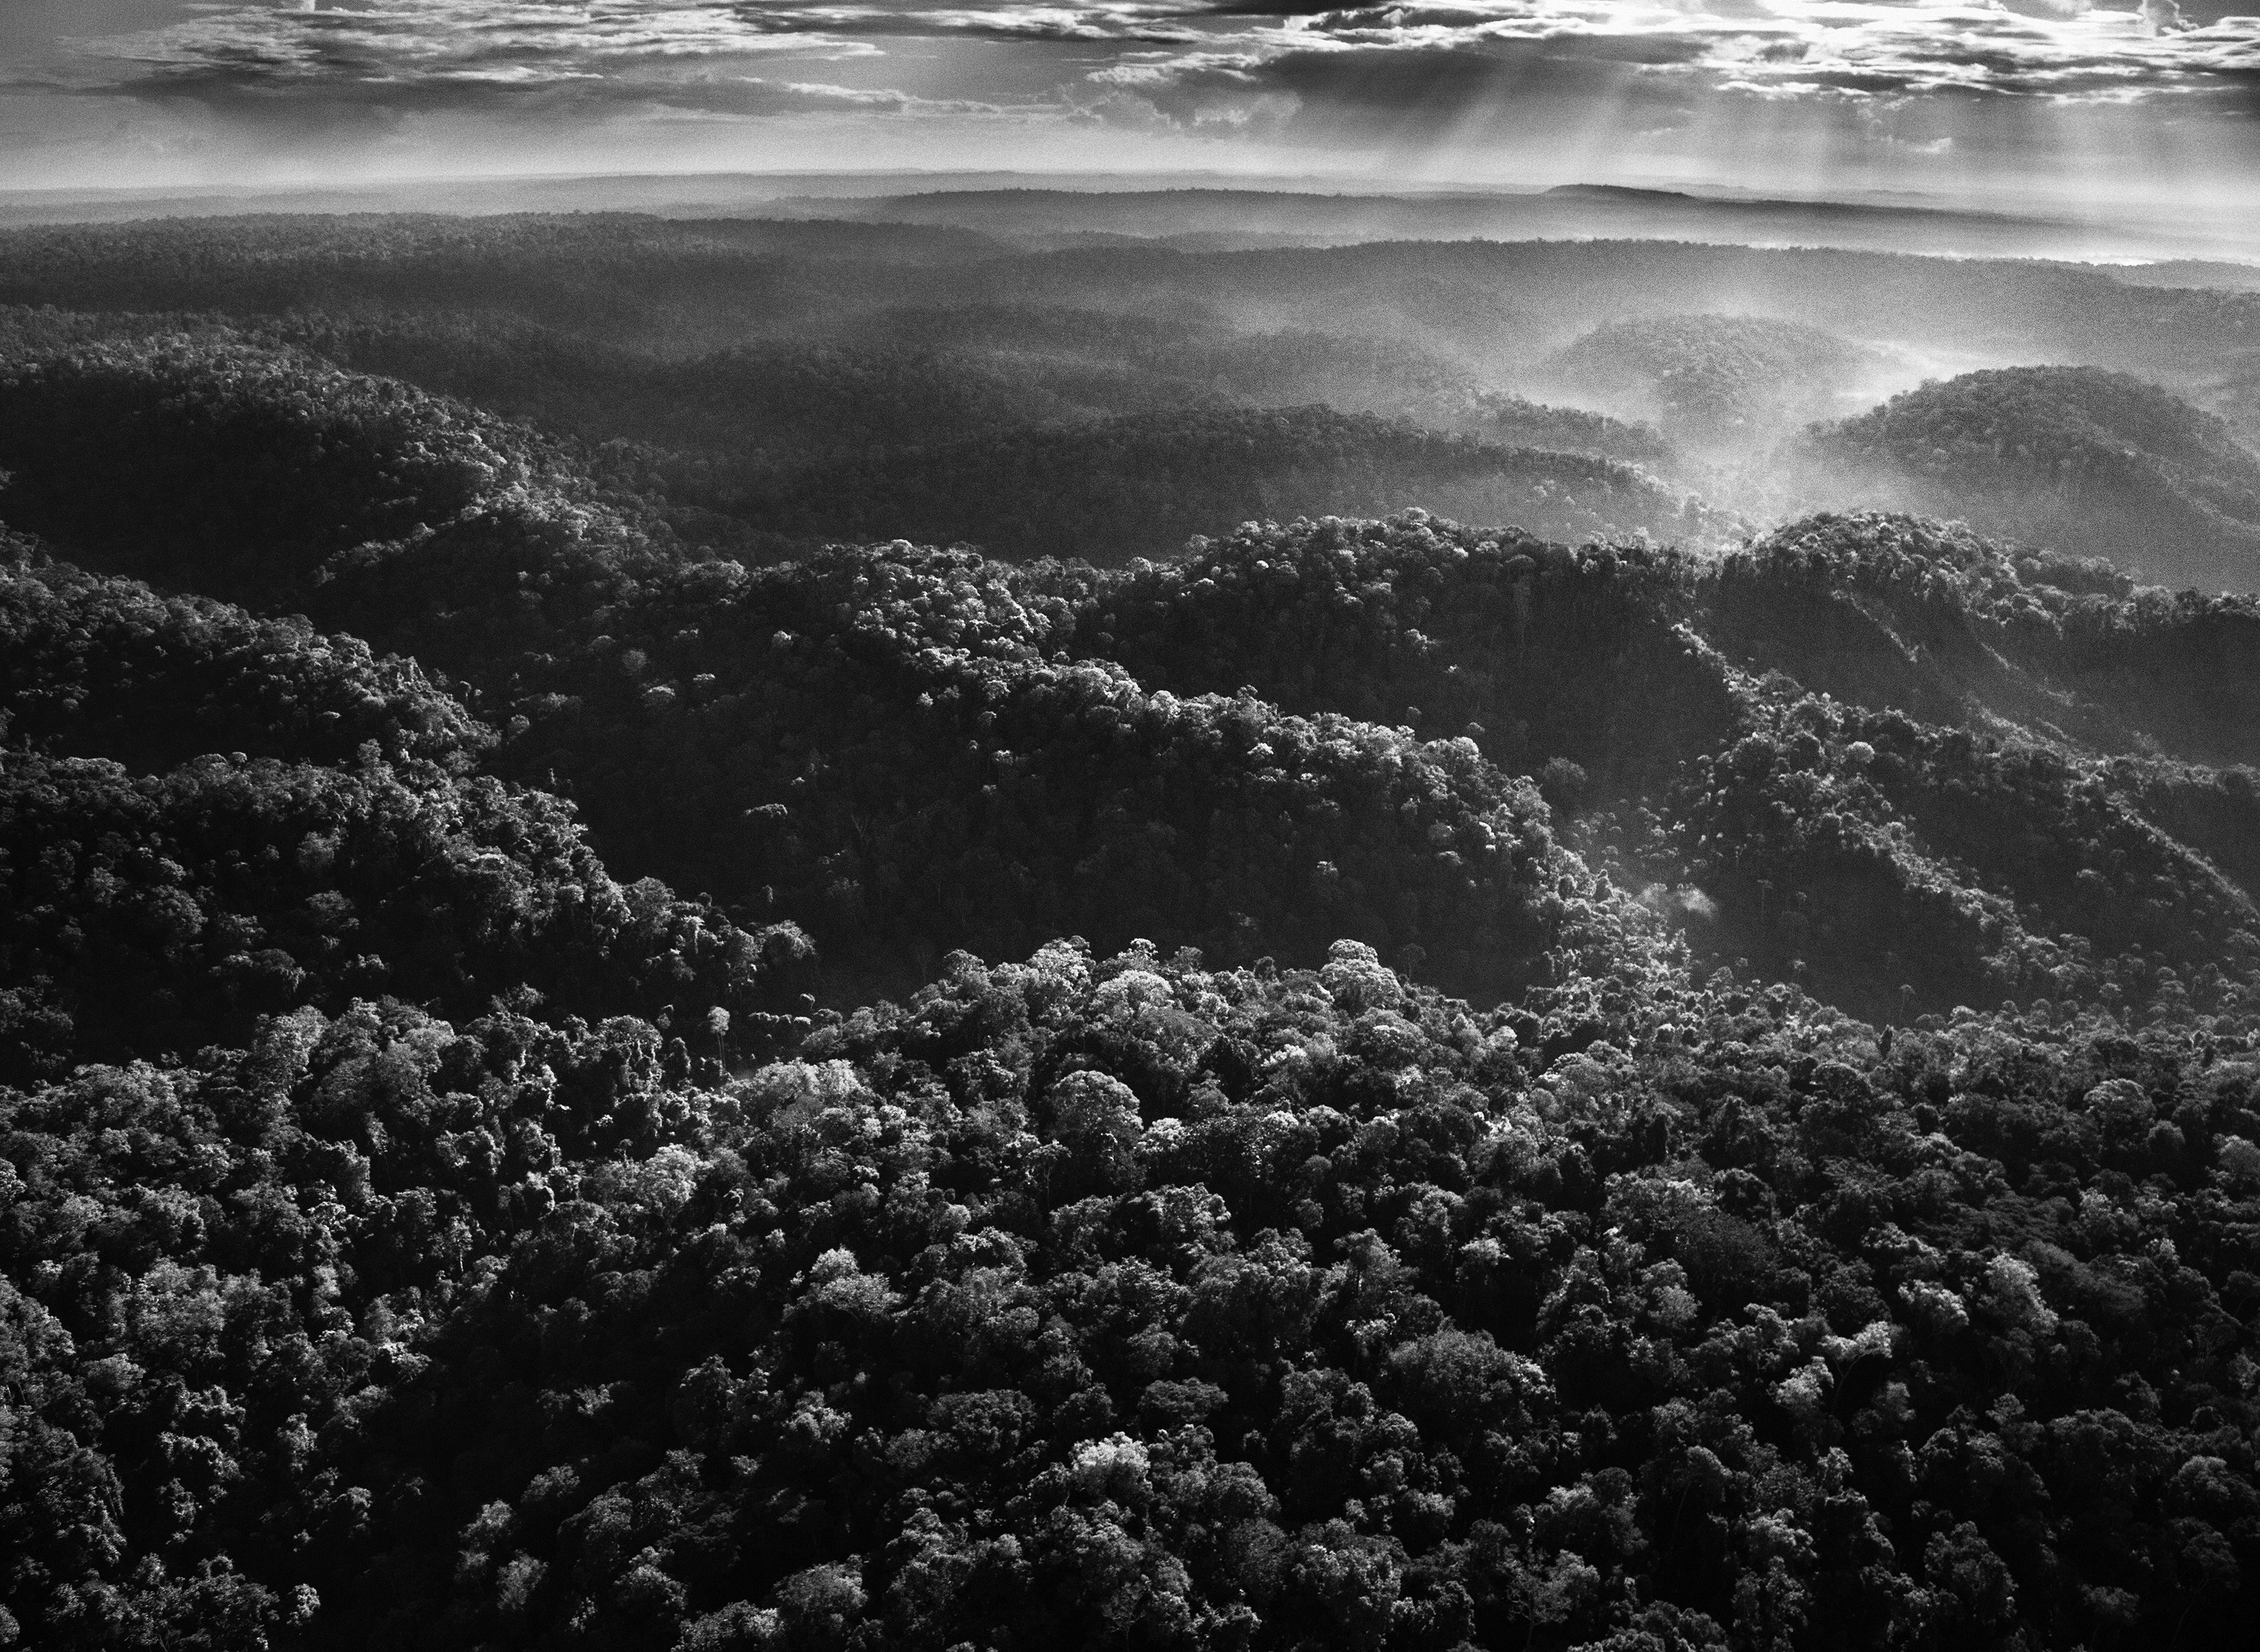
\includegraphics[width=\textwidth]{./imgs/Paisagem_SS}
\caption{Foto aérea de Sebastião Salgado}
\end{figure}

As narrativas do contato passam pela introdução de novos alimentos e a
mudança na dieta. ``Saber comer'' alimentos com farinha ou frangos era
algo que os Guajá desconheciam, e como veremos no decorrer desse livro
alimentos outrora restritos passaram a ser consumidos com mais
frequência enquanto outros deixaram de sê"-lo. Mesmo durante os anos de
fuga, no ``tempo do mato'' (\emph{ka'ape mỹna}), procuravam permanecer
próximos aos cursos dos rios, o que nem sempre era possível. Tinham que
viver nas ``montanhas'' (\emph{wytyra}), onde não há água, e quando
precisavam tomar banho ou pegar água desciam as grandes encostas que os
mantinham seguros, usavam o igarapé mais próximo e retornavam às
``terras altas'' (\emph{wytyra}). Dentre tantos, o principal desconforto
em viver longe de uma fonte de água no meio da floresta era a sede que
experimentavam nesses anos. Esse \emph{tempo da sede} (\emph{haiwe},
``minha sede''), que como lembram era uma ``sede intensa'' ``\emph{iwe
rahy}'', caracteriza os \emph{anos de fuga}, rememorados como \emph{wyhy
ka'a ripi} (``correndo pelo mato''). Nesse tempo, as caçadas eram
difíceis, e para não chamar tanta atenção passaram a ser realizadas à
noite que, como veremos no capítulo 8, no que concerne à caça de
macacos, é algo de extrema dificuldade se for realizado sem luz. Essa
vida nas ``terras altas'' me foi relatada da seguinte maneira por
Akamatỹa:

\begin{quote}
\emph{Nós sempre fugíamos subindo pela montanha. Matávamos capelão e
corríamos para lá. Certa vez, os karai (não"-indígenas) estavam correndo
atrás da gente e nós conseguimos matar apenas um capelão. O capelão
ficou lá em cima da árvore e o matamos à noite, escondido, para os karai
não nos verem. Esperamos lá em cima da montanha e à noite voltamos para
matar capelão escondido. Não tínhamos mais comida, a cabeça doía, e
pensávamos que tínhamos que comer capelão. Os karai nos perseguiam e
tínhamos que ficar fugindo para a montanha. Vimos o rastro dos karai
(não"-indígenas) e fugimos de novo. Quando descíamos, ficávamos só um
pouco e logo tínhamos de fugir de novo. Pensávamos: como vamos viver
assim? Minha mãe, grávida, perdeu um filho porque fez muito esforço,
correndo (pelas terras altas), e ficou com muito medo. Descemos para
procurar babaçu no cocal e ficamos de novo só um pouquinho, depois
fugimos para a montanha. Queríamos muito comer babaçu, mas os karai
estavam lá, nos procurando. Não tínhamos nada para comer. Ficamos lá
escondidos por muito tempo, com sede, com fome e queríamos voltar, mas
os karai estavam lá. Minha mãe ficava muito preocupada: como vamos viver
assim? Vamos tentar ficar aqui escondidos mais um pouquinho, ela dizia.
Eu, que era seu filho, saía de lá para ver se dava para descermos da
montanha, mas encontrava rastro dos karai. Ficávamos sempre fugindo, e
os karai sempre correndo atrás de nós. Minha mãe me falava: como vamos
viver assim? E eu falava: não sei, mãe! Ela dizia, então: vamos ficar
aqui escondidos mais um pouquinho. E ficávamos em cima da montanha, sem
conseguir sair para caçar ou comer babaçu.}
\end{quote}

Nessa época, quando as ``terras altas'' lhes traziam um pouco de
segurança, eram ``gente do mato'', \emph{awa ka'apahara}, e não conheciam
o jeito dos \emph{karai} (brancos). Algumas pessoas queriam aparecer
para o contato com os \emph{karai} enquanto outros resistiam, pois
tinham medo, como certa vez me explicou Kamairua. Não por acaso, é por
meio deste mesmo nome, \emph{awa ka'apahara} (``gente do mato''), que os
Guajá que vivem nas aldeias pensam os pequenos grupos que ainda vivem
sem contato oficial (os ``isolados'', de acordo com a terminologia
vigente). Como veremos no decorrer deste livro, essa vida de fuga e
abstinência é experimentada hoje pelos que se encontram isolados, pois
permanecem como ``gente do mato'', \emph{awa ka'apahara}, e se alimentam
com uma ``comida de gente do mato'' (\emph{awa mihu nimi'ũa}, ``comida
de gente braba'') que as pessoas da aldeia há muito deixaram de
consumir, como um ``cará"-do"-mato'' (\emph{karuhua}), além de um
tubérculo chamado \emph{mara'atỹa} --- que não consegui identificar,
glosado genericamente como uma ``raiz'' ou ``batata do mato''. Esses víveres
eram utilizados como alternativa alimentar durante as fugas. Destaco o
trecho de um depoimento gravado com Kamairua (aldeia Tiracambu) em que
ele relaciona o consumo desse tubérculo à vida nas ladeiras/montanhas, à
falta de cônjuges e à penúria dos anos de fuga:

\begin{quote}
\emph{(\ldots{}) E estávamos fugindo dos karai (não"-índígenas) e não
sabíamos o que comer. Não tinha caça. O que será que vamos comer?,
pensávamos. Vamos comer mara'atỹa. E então comemos mara'atỹa. Arrancamos
e comemos, apesar de ela ser uma raiz muito dura, que dá na montanha.
Nessa época não tinha mulher para casar, não tinha rede. As redes
estragaram e não tinha mais fibra de tucum. Conseguimos um dia matar
capelão e comemos com mara'atỹa (conversa com Kamairua, aldeia
Tiracambu, 2013. Tradução: Uirá Garcia e Marina Magalhães).}
\end{quote}

Ainda sobre a vida em fuga pelas terras altas, Akamatỹa reflete sobre a
penúria alimentar e o \emph{mara'atỹa} em seus anos de fuga:

\begin{quote}
\emph{(\ldots{}) Comíamos só jaboti. Estávamos eu, minha mãe, meu pai,
minha irmã Pakawãja, ainda bebê. Hajkaramykỹ ainda não tinha nascido.
Passamos a comer mara'atỹa (``batata do mato''). Arrancávamos escondido
e comíamos assado. Mas um dia os karai viram a fumaça e nos encontraram
novamente. Mandaram cachorro atrás de nós e tivemos de subir a ladeira
de novo e comer mara'atỹa escondido. Queríamos muito comer babaçu, mas
os karai não deixavam chegarmos ao cocal. Só podíamos comer mara'atỹa
mesmo. Um dia encontramos um outro Awá-Guajá que perguntou para nós o
que estávamos comendo, falamos que só comíamos mara'atỹa por causa da
fuga. Juntamos os grupos, ficamos juntos (Conversa com Akamatỹa,
aldeia Tiracambu, 2013. Tradução: Uirá Garcia e Marina Magalhães).}
\end{quote}

Tal época foi marcada tanto pela dispersão (por um lado) quanto a
reunião de pequenos grupos que outrora se encontravam distantes no
território. Os Guajá tiveram que encontrar estratégias de alianças
(\emph{ruku}, ``estar com/casar'') e criação de filhos (\emph{ixa'á}
``crescer'') para dar conta do grande número de crianças que se tornaram
órfãs devido à morte dos pais por doenças ou assassinato pelos
\emph{karai} (sobretudo durante a década de 1970, quando a região foi
maçicamente ocupada) ou que simplesmente eram deixadas para outros
parentes as criarem. Xiramua, por exemplo, foi encontrado sozinho na
mata ainda criança, sem pai ou mãe durante a década de 1970, por um
grupo liderado por Ximira, cujos parentes viviam nas cabeceiras do
Igarapé do Presídio e fizeram contato entre 1981 e 1983 (Garcia 2013,
p.51). De acordo com um relato de Tatuxa'a (da aldeia Awá), seu pai,
Ximira, encontrou uma criança ainda tão pequena que não sabia falar,
sozinha, na mata. Essa criança era Xiramua, cujos pais haviam sido
assassinados por \emph{karai} (não"-indígenas). Em outro relato,
Akamatỹa, da aldeia Tiracambu, relembra que seu pai ficou para trás
deixando os filhos:

\begin{quote}
\emph{Antes de chegar aqui, meu pai ficou velho e disse: podem correr
na frente meus filhos. Estou velho e não aguento mais. Pode deixar que
me matem. E ele ficou no mato. Uma vez eu pisei de noite em uma
surucucu, que me mordeu. Depois que chegamos aqui nessa região, tentamos
voltar de novo para o nosso antigo lugar, mas já não havia mais mata, só
capoeira (relato de Akamatỹa).}
\end{quote}

Kamairua, que também foi criado sem os pais, reforça os muitos
rearranjos de paternidade que visam à criação de crianças (\emph{ixa'á}
``crescer'') largadas, nos anos de fuga. A partir de si e seu
amigo/germano, Irakatakoa, ele revela.

\begin{quote}
\emph{Antigamente eu vivia no mato. Eu não conheci meu pai e ficava
com minha avó, Mirakexa'a. Da mesma forma que o Irakatakoa, que era bebê
(e foi criado por Marakanã). Tínhamos medo dos karai (não"-indígenas).
Irakatakoa nasceu, e sua mãe morreu de parto. Iam deixá-lo para que os
karai o criassem, mas ficaram com pena, e Marakanã passou a criá-lo.
Quanto a mim, quando eu era pequeno uns karai chegaram e minha avó me
pegou, fugindo deles. Nós vivíamos juntos até que encontramos os karai e
tivemos que nos espalhar. (\ldots{}) Queríamos vir para cá (para o Posto
Indígena Awá), mas tínhamos medo. Então ficávamos no mato, matando
capelão, queixada, moqueávamos queixada, comíamos. Piramỹna, então, se
separou de nós e eu fiquei com minha avó (Mirakexa'a) e Karawaxa'a. Foi
quando os karai (não"-indígenas) apareceram e tivemos de fugir. Minha avó
me pegou, pois eu era bem pequeno, e o meu pai fugiu para outro lado, em
direção ao Turiaçu. Por isso eu não conheci meu pai. Só fui conhecê-lo
há pouco tempo, lá no Turiaçu (na aldeia Guajá). Eu vi meu pai, Tõja
(Kamixaxa'a), depois de adulto. Eu era pequenininho, e foi minha avó
quem me criou. Eu comia ovo de jaboti, eu comia mel, lá na região do
Tabocão. E assim fui crescendo, crescendo até ficar grande (Conversa
com Kamairua, 2013. Tradução: Uirá Garcia e Marina Magalhães).}
\end{quote}

A melancolia dessas lembranças remete aos muitos parentes que morreram,
ao medo dos brancos, a sede e fome, além das cercas de arame farpado que
entrecortavam a terra e delimitavam ``fazendas'', cujos jagunços
(\emph{karai mihua} ``brancos violentos'') realizavam expedições
``punitivas'', matando famílias inteiras. As feridas por arame farpado
colocados como emboscadas para machucar os Guajá, tal Kamairu me
explicou certa vez, aparecem sensivelmente documentadas no filme
\emph{Serras da Desordem}, de Andrea Tonacci. \emph{Xiramukũ} (filho de
Karapirú), que nasceu no mato e se separou da família em uma dessas
fugas após um ataque a tiros a seu grupo, feito pelos \emph{karai} na
região de Porto Franco (Maranhão) em 1978, foi encontrado por moradores
locais preso a uma armadilha de arame farpado feita pelos próprios
jagunços que mataram sua família, por ordem do dono de uma fazenda da
região (Tonacci 2006). Os Guajá, que viviam caminhando e nessa época
corriam em fuga, passaram a encontrar em suas trilhas (\emph{hapea}
``meu caminho'') esse novo obstáculo, o arame farpado, colocado para
feri"-los e, como no caso de \emph{Xiramukũ}, prendê"-los.

Em outra conversa, Irakatakoa e Xipowaha se lembravam de algo não tão
raro na história guajá, que era o encontro com colonos da região que
lhes forneciam utensílios, comida e outros artigos. Há uma história de
contato não"-oficial, bem anterior ao contato com a \versal{FUNAI}, e de acordo
com relatos (cf. Ribeiro 1996; Beghin 1957) e depoimentos, como a
narrativa que abre este livro, esses encontros eram menos ``traumáticos'';
algo como um interesse mútuo entre os Guajá e moradores que viviam
isolados no interior da mata, derrubando a floresta para ``botar'' roça,
no clássico modelo de derrubada, queima e povoamento que marca a
ocupação do Maranhão e de boa parte da Amazônia. Os ocupantes que não
entravam em conflito com os Guajá são lembrados como \emph{karai katy}
(``não"-indígenas calmos/bons'') em oposição a, por exemplo, \emph{karai}
\emph{mihua} (``nervosos/maus''). E a própria \versal{FUNAI}, à época dos
primeiros contatos, era considerada um tipo de \emph{karai katy} (branco
bom), por ofertar utensílios e atrai"-los.

\section{Trabalho, \emph{Trabaio}}

Se no ``tempo do mato'' a dieta era marcada por uma espécie de
sub"-alimentação e caçadas precárias, a chegada dos \emph{karai} mudaria
radicalmente o conteúdo e formas alimentares. A introdução de espécies
cultivadas seria o principal decodificador dessa passagem de \emph{awa
ka'apahara} ``gente do mato'' --- ou \emph{awa mihua} ``gente braba'' ---
para \emph{awa katy}, ``gente mansa'' (ou ``gente da aldeia''), tal como
se pensam hoje em dia. O espanto, receio e curiosidade frente a esses
novos alimentos é refletido por Irakatakoa, da aldeia \emph{Awá}, que se
lembra inclusive de Mercio Gomes (antropólogo --- e ex"-presidente da \versal{FUNAI}
--- que trabalhou com a antiga frente de atração), durante o contato com
seu grupo, realizado na região do Igarapé Timbira, entre 1980 e 1983:

\begin{quote}
\emph{Eu era pequeno. Mas meu pai (Tatajkamaha) conta que Mércio
(chamado aqui de Jakuxa'a) ofereceu arroz para ele dizendo que era muito
gostoso. Meu pai experimentou e cuspiu. Achou muito ruim e ficou bravo
com ele. Aí ele disse que era para meu pai ficar calmo, pois ele era um
``branco bom'' (karai katy). (\ldots{}) Ele ia nos levar para lá (\versal{PIN} Awá)
para nos amansar, para aprender a comer sal, açúcar, café. E meu pai
experimentava e cuspia, jogava tudo fora. Aí um dia, o Piramỹna
experimentou e gostou. E Mércio disse que íamos nos acostumar e que ia
ficar tudo bem conosco lá. Ia ter arroz, feijão, abóbora, cebola. Mas
tudo o que provávamos, jogávamos fora. E nos escondíamos novamente no
mato. Aí o Major (apelido de um antigo), ia atrás de novo. Alguns de nós
ficavam tremendo de medo. E ele dizia: --- não vamos te matar não,
queremos que vocês se acostumem conosco. Eu também tinha muito medo.
Chorava e fazia cocô. Porque eu não conhecia branco. Aí Mércio disse que
seria bom pra mim. Aí eu fiquei acostumado e vim para cá, com todos os
outros. Já estavam aqui o Ximira e o Urixia. Eles já tinham nos avisado
que teriam outros Awá-Guajá aqui também. Estavam também o Mitũa, o
Kamana'ĩa. E minha avó, que veio conosco (a falecida Mirakexa'a), já
conhecia eles todos (de uma época anterior ao contato) (Conversa com
Irakatakôa, Aldeia Awá, 2013. Tradução: Uirá Garcia e Marina Magalhães).}
\end{quote}

Os relatórios da Frente de Atração reportam sobre a compra de farinha de
mandioca a ser fornecida aos grupos contatados na década de 1980, algo
que logo se tornou insustentável, obrigando as aldeias que se formaram a
produzir a própria farinha em um regime de trabalho coordenado pela
\versal{FUNAI}, o que, rapidamente, fez com que a farinha de mandioca puba se
tornasse a base da dieta.

Em todas as jornadas de caça, a farinha é um item essencial, não existem
caçadas sem que levem ao menos uma pequena quantidade de farinha para a
floresta. Quando estão em seus acampamentos de caça por muitos dias ou
semanas, sempre haverá alguém na aldeia torrando mais farinha para ser
levada ao acampamento. Na alimentação cotidiana isso também é sentido,
os Awá adicionam farinha a praticamente todos os alimentos que consomem
(abóbora, coco de babaçu, inajá, bacaba e açaí), além de ela ser usada
para fazer mingaus a partir dos caldos de carnes, peixes e legumes. O
reflexo desta não intimidade com o trabalho agrícola --- bem diferente de
seus vizinhos Ka'apor e Guajajara --- pode ser visto, por exemplo, na
falta de assiduidade com que Guajá mantêm suas roças, muitas das quais
têm a colheita seriamente prejudicada. De acordo com Forline:

\begin{quote}
\emph{As roças normalmente exigem um ciclo de atividades que tem que ser
seguido conforme o calendário metereológico e ecológico. Isso implica na
limpeza, derrubada, queima, coivara, plantio, colheita e capinagem.
Segundo estimativas de alguns funcionários da \versal{FUNAI}, os Guajá não têm um
aproveitamento total (ou máximo) de suas roças, perdendo até 60\% de sua
produção, dado que ainda não têm a experiência que seus vizinhos possuem
na agricultura e ainda dedicam mais tempo de suas atividades produtivas
à caça, situação essa que não antecipa muito a sucessão florestal e o
avanço das capoeiras (Forline 2007, p.6).}
\end{quote}

Em suma, mesmo havendo hoje em dia o cultivo agrícola nas aldeias ---
sempre com a ajuda de mão de obra contratada pela \versal{FUNAI} ---, ainda não
podemos afirmar que os Awá sejam algo como \emph{horticultores}, no
sentido que a ecologia política atribui a essa ideia, embora seja
possível identificar um processo de incorporação da agricultura à vida.
A lógica de ação é baseada na caça, e todos ainda estão dispostos a
trocar uma colheita coordenada pela \versal{FUNAI} pela floresta, a partir de uma
mera suspeita da existência de uma vara de porcos ou um bando de
capelães.

Com isso, deparamo"-nos com uma \emph{missão civilizadora} por parte do
órgão indigenista para transmitir/ensinar o trabalho agrícola para os
Guajá. Até os dias atuais, observa"-se na fala de funcionários da \versal{FUNAI}
que convivem diretamente com eles a preocupação que norteou os anos de
contato --- e que permeia inclusive as políticas de contato atual ---, que é
o medo de os grupos recém"-contatados morrerem por inanição ao se
recusarem a consumir os alimentos introduzidos pelos brancos, já que há
dificuldade em manter a antiga dieta, do ``tempo do mato''. Assim, na
época da frente de atração (até a década de 1990), o posto indígena
tornou"-se uma espécie de unidade produtiva, mantendo com as aldeias uma
relação que passava fundamentalmente por comando e ordem, tal uma
``colônia agrícola'' ou algo do gênero (cujos resquícios são sentidos
até os dias atuais). Sugiro aqui que tal relação possa ser pensada a
partir da ideia de ``trabalho'', tal como observa"-se há décadas pelos
funcionários da \versal{FUNAI}, a partir de ideias como ``\emph{os índios
precisam aprender a trabalhar}'', ou ``\emph{os índios não sabem
trabalhar}'', ou mesmo que ``\emph{se não trabalharem esses índios vão
morrer de fome}''. A figura do ``trabalho'', tal como coordenado pela
\versal{FUNAI}, com contratação de mão de obra de moradores do entorno da terra
indígena para ajudá"-los, é traduzida pelos Guajá mediante a ideia de
\emph{trabaio}, que --- como experimentei na aldeia Juriti onde vivi
durante o meu doutorado --- pode ser considerada algo diferente de
``trabalho''. Por exemplo, pronunciar palavrões em português, soltar
gritos e um monte de jargões do tipo ``\emph{eu sou trabalhador!}'' ou
``\emph{eu sou duro!}'' dentre outros, compõe uma sociabilidade
masculina experimentada no trabalho de roça dos \emph{karai} e
atualizada pelos Guajá a partir da ideia de \emph{trabaio}. Eu mesmo
passei excelentes momentos junto aos homens nessas atividades que
misturam a alegria de estarem juntos com seus amigos e com os
\emph{karai} da \versal{FUNAI} (\emph{karai katy}, ``brancos bons''), momentos em
que visivelmente os Guajá --- de muitas formas --- imitavam os \emph{karai},
tentando entender um pouco mais sobre eles.

Um conjunto de elementos e ações define o \emph{trabaio} (ou
\emph{trapaio}, a depender da pronúncia) que ocorre fundamentalmente na
lavoura. Para ir à roça, um homem, além de ferramentas como facões e
terçados, exige roupas (calça comprida, botina, boné e camisa de manga
longa para se proteger), o mesmo tipo de vestimenta que os \emph{karai}
(os brancos) utilizam no trabalho na roça. Vestir roupas de branco faz
parte do \emph{trabaio} da mesma forma que beber a água gelada do posto
da \versal{FUNAI} levada pelos funcionários para a roça; perguntar e comentar
detalhes íntimos da vida em casal, em tom de provocação; e,
principalmente, consumir a comida dos \emph{karai}. Em uma conversa que
tive com Irakatakoa, da aldeia \emph{Awá}, ele afirma precisar comer a
comida do branco (\emph{karai nimi'ũa}) --- arroz, macarrão, carnes e
sardinhas em lata --- quando vai para a roça: ``\emph{É assim que os
brancos trabalham na roça. Suas mulheres preparam a comida e os homens
levam a comida para a roça, por isso é assim que deve ser o trabalho dos
Guajá. Com comida nós vamos para a roça}''. Na tentativa de estimular
atividades de roça para os Guajá da \versal{TI} Caru, a Frente de Proteção
cogitou inclusive pagar uma espécie de ``bônus'' por cada linha de
roça\footnote{No estado do Maranhão as roças são medidas por ``linhas'',
  cada linha equivale a 0,30 hectare.} cultivada, além de se encarregar
de levar o ``rancho'' a cada jornada na lavoura.

Se a política oficial atual é não oferecer mais nada do que se oferecia
nas décadas anteriores (farinha, sal, sabão, munição etc.), pouca coisa
mudou desde então, e a procurada autonomia para o ``trabalho'' não vem
ocorrendo como se esperava no passado. É comum os funcionários da \versal{FUNAI}
reclamarem da dificuldade em ``juntar três ou quatro homens para o
trabalho''. Por exemplo, em 2012, a grande aldeia ligada ao posto
indígena \emph{Awá}, por falta de comunicação e organização desses
trabalhos não fez nenhuma roça, e em 2013 foi necessário que a própria
\versal{FUNAI} comprasse toneladas de farinha e partes cultivadas por
agricultores próximos para dar conta das necessidades da aldeia. No
entanto, esse descompasso que ainda existe na vida das pessoas, como
veremos, se deve à diferença de estatuto entre a caça e a ``comida de
gente'' (\emph{awa nimi'ũa}) e a comida dos não"-indígenas (\emph{karai
nimi'ũa)}. Os Guajá reclamam que seus filhos e mulheres têm fome, que
precisam caçar para eles, e que quando vão para a roça não conseguem
realmente caçar. Não à toa, são capazes de quebrar qualquer acordo
prévio que tenham feito com os funcionários do posto indígena e de
trocar a lavoura por uma promessa de caça, seja por alguém ter
encontrado um rastro ou serem informados por um sonho, ou mesmo para
suprir o desejo de uma mulher, um filho ou até um sogro, para desespero
dos servidores que os arregimentavam para o trabalho e encontram nesses
momentos um sinal da própria \emph{inconstância} Guajá. Ir para a roça
nesses casos é, antes de tudo, sinônimo de não ir caçar.

A floresta, por sua vez, seria o oposto do \emph{trabaio}, fresca e
cheia de imprevisibilidade, ela se distingue frontalmente das aldeias e
roças, locais quentes e monótonos se comparados à floresta. Acostumados
à vida no interior da mata, sempre ``fresca'' (\emph{haxỹ}), a
exposição ao sol por muitas horas é algo considerado bastante
desagradável. Um dos componentes, portanto, que agenciaria essa ideia de
\emph{trabaio} passa pela possibilidade de suportarem o calor do sol
(\emph{kwarahy haku}). Ser forte (\emph{hatỹ}, ``duro'') no trabalho
significa aguentar o trabalho de sol"-a"-sol, tal como valorizado pelos
\emph{karai} (brancos) e anteriormente desprezado pelos Guajá. É comum
ouvirmos de uma aldeia para outra que naquele local eles sabem trabalhar
pois são mais ``duros'' e seus corpos aguentam o sol, diferente de
outras aldeias onde as pessoas ainda seriam ``selvagens'' (\emph{awa
ka'apahara} ``gente do mato'') e moles para o trabalho.

Podemos pensar que ``trabalho'' aqui seria mais uma daquelas noções como
``dinheiro'', ``desenvolvimento'', ``lucro'', ``produção'', ``higiene'',
``educação'', ``lazer'', ``alma'', dentre tantas outras levadas aos
povos não"-ocidentais a partir do aparelho colonial, ao mesmo tempo que
reviradas e repensadas por esses povos (Sahlins 1997, Wagner 1981, p.
31--33). Parafraseando a ideia melanésia de \emph{divelopman},
desenvolvida pelos Agamen da Nova Guiné (Nihil 1989 \emph{apud} Sahlins 1997a,
p.59), \emph{trabaio} ``é um conceito amplo'' entre os Guajá --- avaliado
sobretudo a partir das mudanças experimentadas na passagem de um tipo de
gente \emph{awa ka'apahara} (gente da floresta'') para outro tipo de
gente \emph{awa katy} (``gente mansa''/ ``gente da aldeia'').
\emph{Trabaio} aqui seria a tradução de um estilo de vida, e não apenas
``trabalhar''. Sem dúvida, o ``trabalho'' também é contemplado por essa
ideia, que sugere algo mais do que ``trabalhar'', traduzindo o próprio
jeito de viver dos não"-indígenas. Por exemplo, quando eu estava em casa
e demorava para retornar à aldeia Juriti meus amigos sabiam tratar"-se de
\emph{trabaio}, que incluía também andar de avião, dirigir automóveis,
cuidar de uma família com mulher e filhos, comer comida de branco,
enfim, viver como um autêntico \emph{karai}.

De alguma forma o \emph{trabaio} é tudo o que os Guajá não
experimentavam antes do contato, e toda transformação vivida
recentemente pelas pessoas das aldeias --- interessados agora em dinheiro,
escola, carteira de motorista, dentre outros serviços e bens
estrangeiros --- passa pela ideia de que os \emph{karai} (brancos)
``trabalham'' para terem essas coisas, ao passo que os Guajá ainda não
saberiam ``trabalhar'' (na roça, por exemplo). Ao menos na aldeia
Juriti, o \emph{trabaio} é também um compromisso de atividades com a
\versal{FUNAI} que os restringiria em sua vida na floresta. Para as pessoas dessa
aldeia não se trata apenas de ``trabalhar'' nas roças, pomares e áreas
onde é preciso capinar, como orientam os funcionários do posto, o
\emph{trabaio} engloba um conjunto de problemas, dilemas e diferenças
que pautam a própria relação entre os Guajá e os brancos. O conhecimento
que temos das máquinas, o desprezo que temos pela floresta e pelos
conhecimentos indígenas, a brutalidade e grosseria presentes nas
relações entre amigos do sexo masculino (algo deveras chocante para os
homens Guajá), a divisão do tempo, a dieta, o mundo do dinheiro, enfim,
é a própria vida dos \emph{karai/}brancos (chamemos de \emph{sociedade})
que é traduzida pela ideia de \emph{trabaio}. Algo como o \emph{kago}
melanésio (Wagner 1981 p.31), \emph{trabaio} seria a contraparte Guajá
para ideias como ``qualidade de vida'' ou mesmo ``cultura''.
\emph{Trabaio} é a palavra \emph{neo"-guajá} para a experiência de
\emph{virar branco} (Kelly 2005) que revela ``um processo --- um momento
passageiro de ``primeiro contato'' que pode bem durar mais de cem anos''
(Sahlins 1997, p.60). Parafraseando Roy Wagner, \emph{trabaio}
funcionaria como ``um termo de mediação entre diferentes povos'', e ``a
relação que ele encarna'' torna"-se aquela dos Guajá com a sociedade
nacional e com o próprio ocidente (Wagner 1981 p.32).
